\begin{componente}{CLIPS}
\compDescrizione{package generale contenente il prodotto del progetto}
\begin{compPackageContenuti}
\item CLIPS::client: componente globale per il front end del prodotto che utilizza il design pattern \gl{MVC}. Si occupa di fornire un'interfaccia grafica dell'applicazione e di interagire con il lato server.
\item CLIPS::server: componente globale per il back end del prodotto
\end{compPackageContenuti}
\end{componente}
\begin{componente}{CLIPS::client}
\begin{figure}[h!] 
\centering 
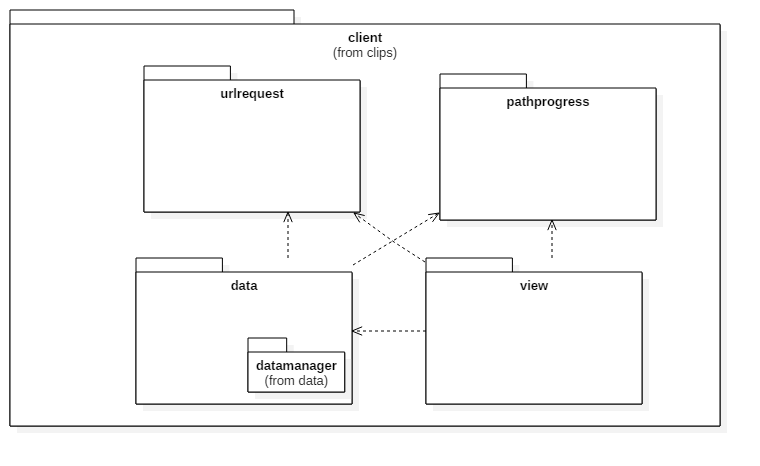
\includegraphics[scale=0.4]{img/package/png/client.png} 
\caption{Schema package client} 
 \end{figure} 
\compDescrizione{componente globale per il front end del prodotto che utilizza il design pattern \gl{MVC}. Si occupa di fornire un'interfaccia grafica dell'applicazione e di interagire con il lato server.}
\compPadre{CLIPS}
\begin{compPackageContenuti}
\item CLIPS::client::data: package per la gestione in locale dei dati
\item CLIPS::client::pathprogress: componente che gestisce i dati del percorso e salva i risultati ottenuti nelle prove mentre si sta giocando
\item CLIPS::client::viewcontroller: componente che raggruppa tutte le view ed i controller relativi alle view
\end{compPackageContenuti}
\end{componente}
\begin{componente}{CLIPS::client::data}
\begin{figure}[h!]
	\centering
	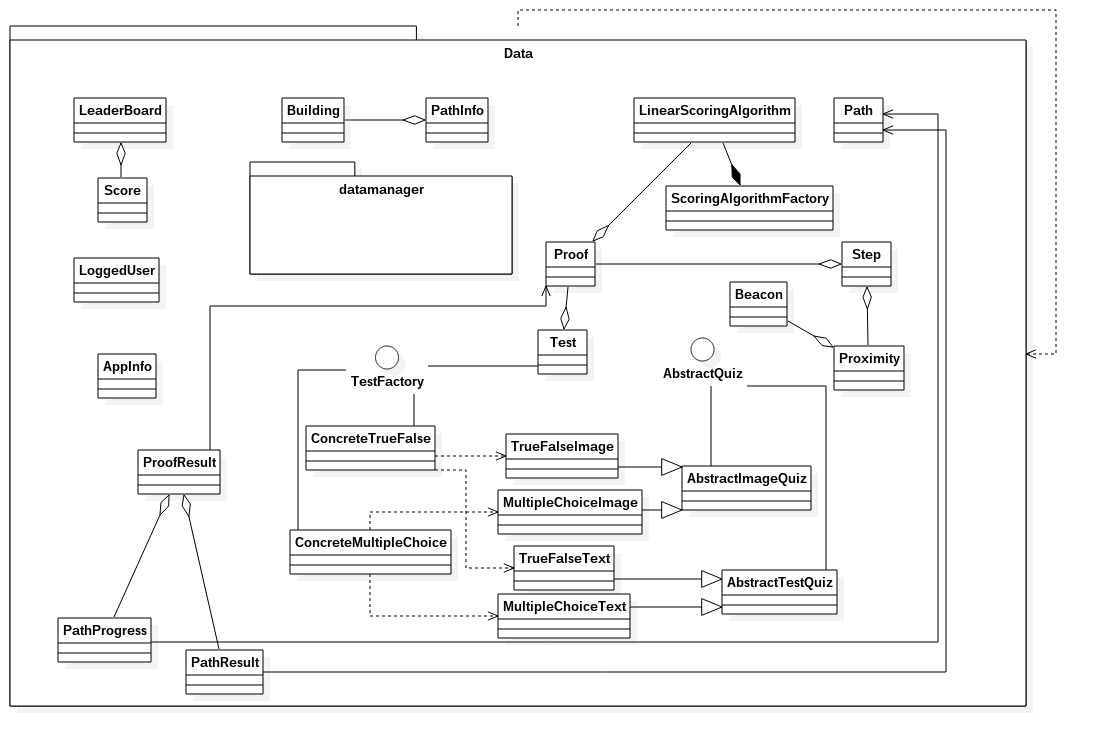
\includegraphics[scale=0.35]{img/package/png/client--data--min.png}
	\caption{Schema sintetico package client::data}
\end{figure}
\begin{figure}[h!]
	\centering
	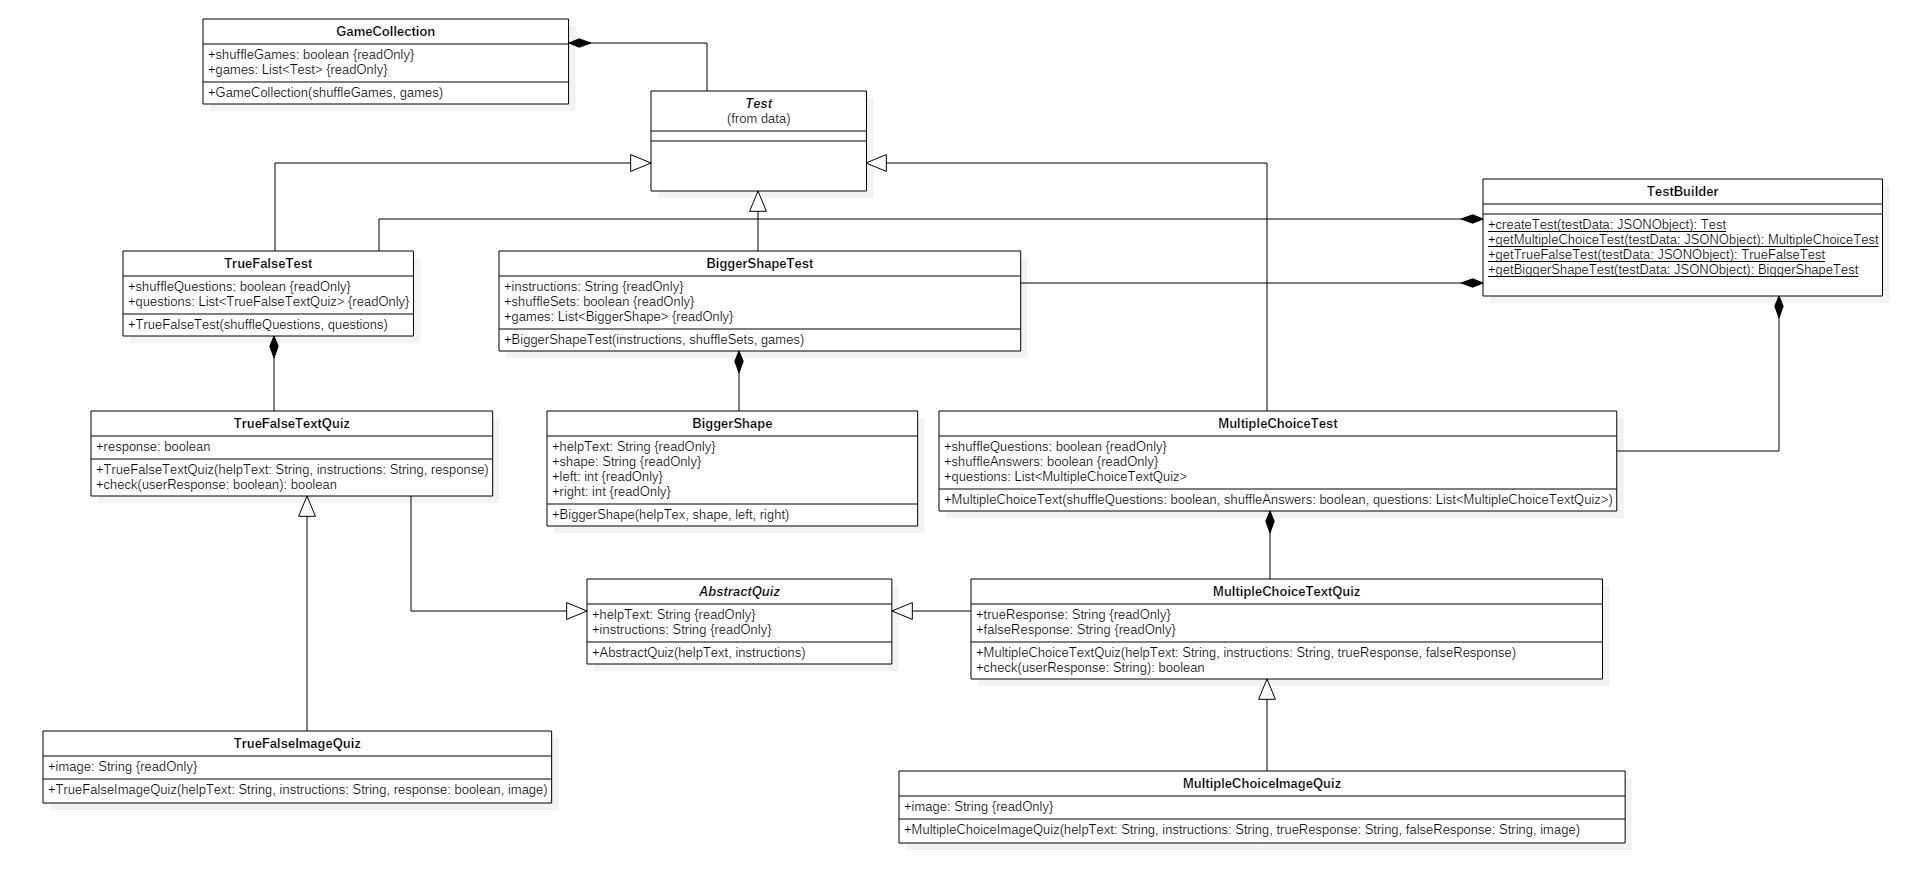
\includegraphics[scale=0.35]{img/package/png/client--data1.png}
	\caption{Prima parte schema package client::data}
\end{figure}
\begin{figure}[h!]
	\centering
	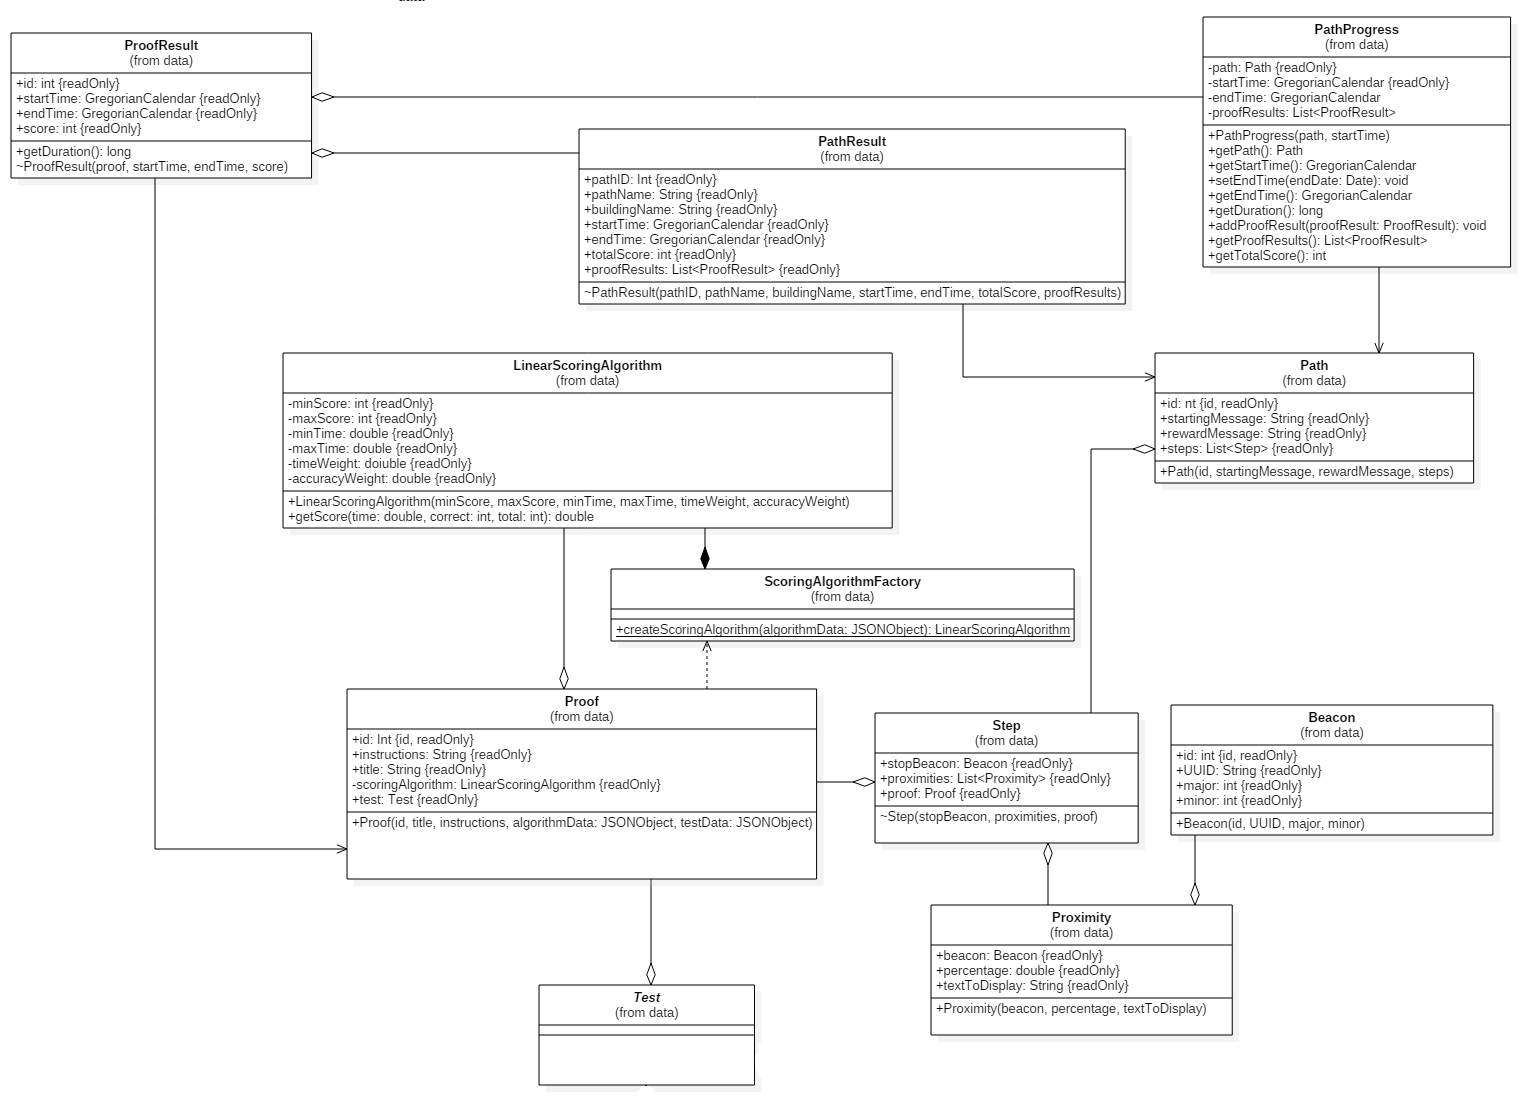
\includegraphics[scale=0.35]{img/package/png/client--data2.png}
	\caption{Seconda parte schema package client::data}
\end{figure}
\begin{figure}[h!]
	\centering
	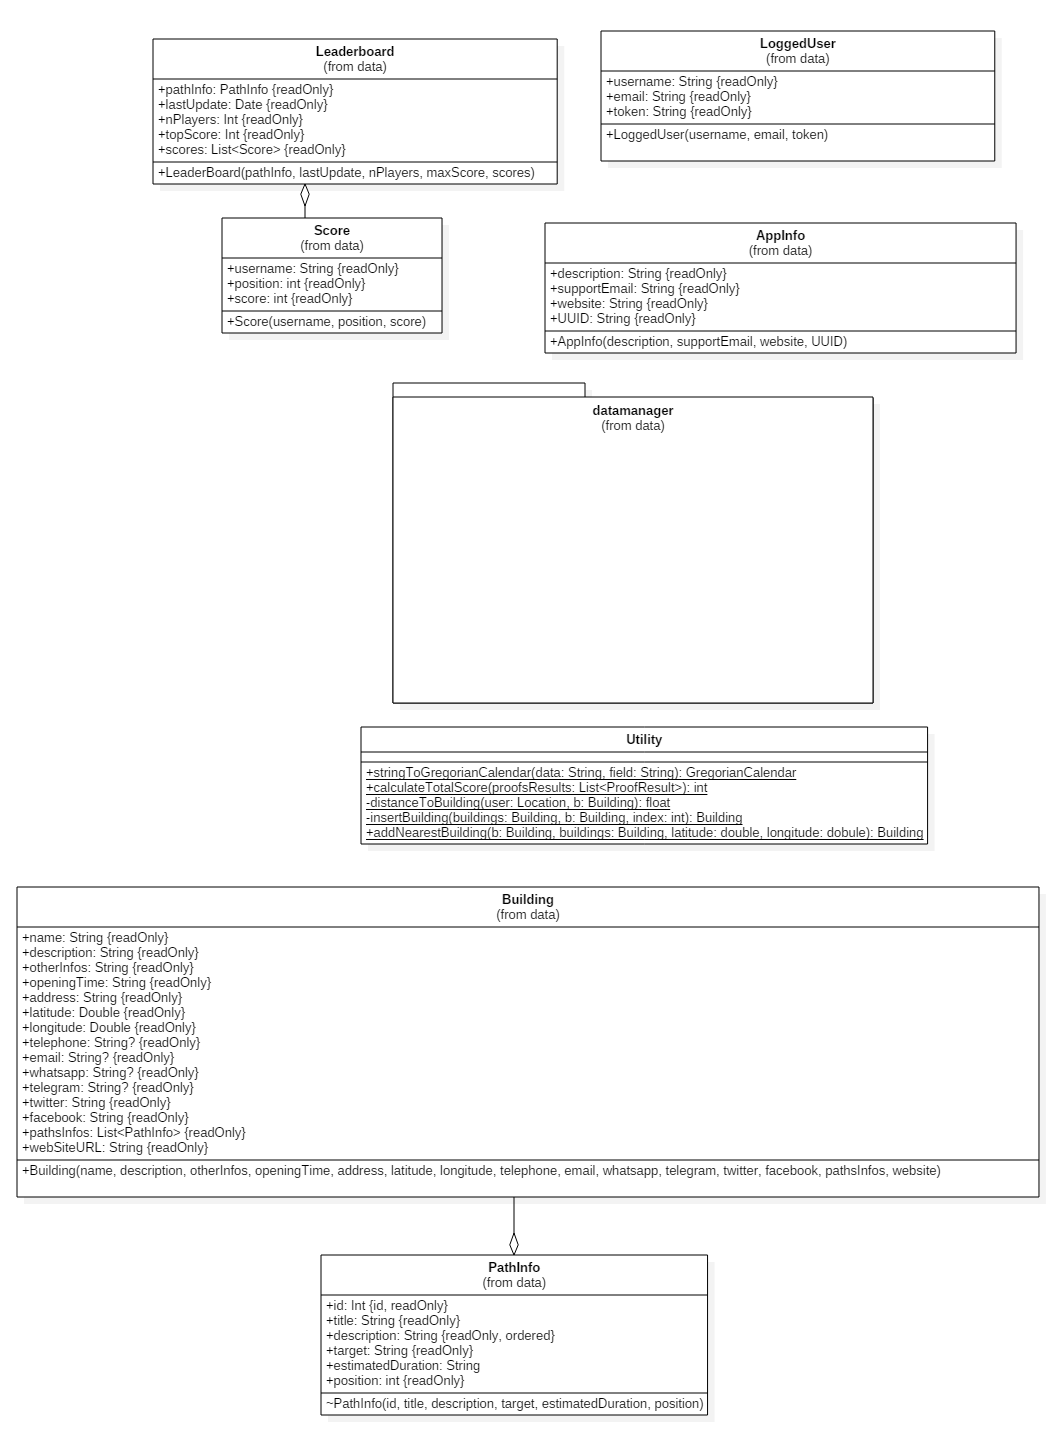
\includegraphics[scale=0.4]{img/package/png/client--data3.png}
	\caption{Terza parte schema package client::data}
\end{figure}
\compDescrizione{package per la gestione in locale dei dati}
\compPadre{client}
\begin{compPackageContenuti}
\item CLIPS::client::data::datamanager: componente che gestisce i dati in locale
\item CLIPS::client::data::urlrequest: componente che si occupa di effettuare le richieste al server
\end{compPackageContenuti}
\begin{compClassi} \\ 
\begin{classe}{CLIPS::client::data::/textit{AbstractQuiz}}
\classeDescrizione{classe astratta per la definizione di un quiz da proporre all'utente}
\classeUtilizzo{classe astratta da cui far derivare tutte le classi che rappresentano un quiz}

\end{classe}\begin{classe}{CLIPS::client::data::/textit{Test}}
\classeDescrizione{classe astratta che rappresenta la definizione di un test da proporre all'utente}
\classeUtilizzo{classe astratta per rappresentare un test, ovvero un gruppo di giochi generalmente dello stesso tipo}
\end{classe}\begin{classe}{CLIPS::client::data::AppInfo}
\classeDescrizione{classe per la rappresentazione delle informazioni generali dell'applicazione}
\classeUtilizzo{permette di salvare le informazioni generali relative all'applicazione}

\end{classe}\begin{classe}{CLIPS::client::data::Beacon}
\classeDescrizione{classe che rappresenta i dati di un beacon in locale}
\classeUtilizzo{permette di salvere in locale le informazioni di un beacon}
\end{classe}\begin{classe}{CLIPS::client::data::BiggerShape}
\classeDescrizione{classe che rappresenta un gioco in cui bisogna selezionare la figura più grande tra le due che appaiono}
\classeUtilizzo{classe per rappresentare un gioco in cui l'utente deve selezionare la figura più grande tra le due che compaiono}

\end{classe}\begin{classe}{CLIPS::client::data::BiggerShapeTest}
\classeDescrizione{classe che rappresenta un test di BiggerShape}
\classeUtilizzo{classe per rappresentare un test di BiggerShape}

\begin{classeRelazioni}
\classeRelazione{CLIPS::client::data}{BiggerShape}{classe che rappresenta un gioco in cui bisogna selezionare la figura più grande tra le due che appaiono}\end{classeRelazioni}
\end{classe}\begin{classe}{CLIPS::client::data::Building}
\classeDescrizione{classe che rappresenta i dati di un edificio in cui è possibile utilizzare l'applicazione}
\classeUtilizzo{permette di memorizzare i dati di un edificio in locale}
\begin{classeRelazioni}
\classeRelazione{CLIPS::client::data}{PathInfo}{classe che si occupa di salvare in locale le informazioni generali di un percorso}\end{classeRelazioni}
\end{classe}\begin{classe}{CLIPS::client::data::GameCollection}
\classeDescrizione{classe che rappresenta un insieme di test}
\classeUtilizzo{classe per rappresentare un test in cui sono contenuti più tipi di giochi, di fatto è un test che contiene altri test}
\begin{classeRelazioni}
\classeRelazione{CLIPS::client::data}{/textit{Test}}{classe astratta che rappresenta un test}\end{classeRelazioni}
\end{classe}\begin{classe}{CLIPS::client::data::LeaderBoard}
\classeDescrizione{classe che rappresenta la classifica di un percorso di un determinato edificio}
\classeUtilizzo{consente di salvare i dati della classifica in locale}
\begin{classeRelazioni}
\classeRelazione{CLIPS::client::data}{PathInfo}{classe che si occupa di salvare in locale le informazioni generali di un percorso}\classeRelazione{CLIPS::client::data}{Score}{classe che rappresenta il risultato nella classifica di uno specifico percorso svolto dall'utente}\end{classeRelazioni}
\end{classe}\begin{classe}{CLIPS::client::data::LinearScoringAlgorithm}
\classeDescrizione{classe per calcolare il punteggio di una prova}
\classeUtilizzo{si occupa di calcolare il punteggio utilizzando un algoritmo lineare}
\end{classe}\begin{classe}{CLIPS::client::data::LoggedUser}
\classeDescrizione{classe che si occupa di memorizzare in locale i dati dell'utente che ha eseguito l'accesso}
\classeUtilizzo{permette il salvataggio in locale dei dati di un utente loggato}

\end{classe}\begin{classe}{CLIPS::client::data::MultipleChoiceImageQuiz}
\classeDescrizione{classe che rappresenta una domanda a risposta multipla con immagine}
\classeUtilizzo{classe per rappresentare una domanda a risposta multipla in cui viene usata un'immagine per la formulazione del quesito}

\end{classe}\begin{classe}{CLIPS::client::data::MultipleChoiceTest}
\classeDescrizione{classe che rappresenta un test di domande a risposta multiple}
\classeUtilizzo{classe per rappresentare un test di domande a risposta multipla, con immagine o senza}

\begin{classeRelazioni}
\classeRelazione{CLIPS::client::data}{MultipleChoiceTextQuiz}{classe che rappresenta una domanda a risposta multipla}\end{classeRelazioni}
\end{classe}\begin{classe}{CLIPS::client::data::MultipleChoiceTextQuiz}
\classeDescrizione{classe che rappresenta una domanda a risposta multipla}
\classeUtilizzo{classe per rappresentare una domanda a risposta multipla il cui contenuto è solo testo}
\end{classe}\begin{classe}{CLIPS::client::data::Path}
\classeDescrizione{classe che si occupa di salvare in locale i dati riguardanti un percorso di un determinato edificio}
\classeUtilizzo{permette di salvare i dati di un percorso in locale}
\begin{classeRelazioni}
\classeRelazione{CLIPS::client::data}{Step}{classe che rappresenta in locale lo spostamento da una prova a quella successiva}\end{classeRelazioni}
\end{classe}\begin{classe}{CLIPS::client::data::PathInfo}
\classeDescrizione{classe che si occupa di salvare in locale le informazioni generali di un percorso}
\classeUtilizzo{consente di salvare in locale le informazioni generali di un percorso}
\end{classe}\begin{classe}{CLIPS::client::data::PathProgress}
\classeDescrizione{classe per il salvataggio in locale del progresso di un percorso svolto dall'utente}
\classeUtilizzo{permette di salvare in locale i risultati delle prove durante lo svolgimento del percorso}
\begin{classeRelazioni}
\classeRelazione{CLIPS::client::data}{Path}{classe che si occupa di salvare in locale i dati riguardanti un percorso di un determinato edificio}\classeRelazione{CLIPS::client::data}{ProofResult}{classe che rappresenta il risultato di una prova svolta dall'utente}\end{classeRelazioni}
\end{classe}\begin{classe}{CLIPS::client::data::PathResult}
\classeDescrizione{classe che rappresenta i risultati di un percorso svolto dall'utente}
\classeUtilizzo{permette di salvare i dati di un percorso in locale}
\begin{classeRelazioni}
\classeRelazione{CLIPS::client::data}{ProofResult}{classe che rappresenta il risultato di una prova svolta dall'utente}\end{classeRelazioni}
\end{classe}\begin{classe}{CLIPS::client::data::Proof}
\classeDescrizione{classe che rappresenta una prova da proporre all'utente che sta svolgendo un percorso}
\classeUtilizzo{salva in locale i dati della prova da far visualizzare all'utente}

\begin{classeRelazioni}
\classeRelazione{CLIPS::client::data}{/textit{Test}}{classe astratta che rappresenta un test}\classeRelazione{CLIPS::client::data}{LinearScoringAlgorithm}{classe per calcolare il punteggio di una prova}\classeRelazione{CLIPS::client::data}{ScoringAlgorithmFactory}{classe base per la creazione degli algoritmi per il calcolo del punteggio di una determinata prova}\end{classeRelazioni}
\end{classe}\begin{classe}{CLIPS::client::data::ProofResult}
\classeDescrizione{classe che rappresenta il risultato di una prova svolta dall'utente}
\classeUtilizzo{permette di salvare in locale il risultato di una prova}
\begin{classeRelazioni}
\classeRelazione{CLIPS::client::data}{PathProgress}{classe per il salvataggio in locale del progresso di un percorso svolto dall'utente}\classeRelazione{CLIPS::client::data}{PathResult}{classe che rappresenta i risultati di un percorso svolto dall'utente}\classeRelazione{CLIPS::client::data}{Proof}{classe che rappresenta una prova del percorso}\end{classeRelazioni}
\end{classe}\begin{classe}{CLIPS::client::data::Proximity}
\classeDescrizione{classe che rappresenta in locale un beacon dedicato alla segnalazione della distanza dalla prossima prova}
\classeUtilizzo{consente di salvare un beacon e la sua distanza dal beacon della prossima prova}
\begin{classeRelazioni}
\classeRelazione{CLIPS::client::data}{Beacon}{classe che rappresenta un beacon in locale}\end{classeRelazioni}
\end{classe}\begin{classe}{CLIPS::client::data::Score}
\classeDescrizione{classe che rappresenta il risultato nella classifica dell'utente}
\classeUtilizzo{permette di memorizzare il punteggio e la posizione in classifica dell'utente}
\end{classe}\begin{classe}{CLIPS::client::data::ScoringAlgorithmFactory}
\classeDescrizione{classe base per la creazione degli algoritmi di calcolo del punteggio di una determinata prova}
\classeUtilizzo{fornisce il metodo per la creazione di algoritmi per il calcolo dei punteggi}
\begin{classeRelazioni}
\classeRelazione{CLIPS::client::data}{LinearScoringAlgorithm}{classe per calcolare il punteggio di una prova}\end{classeRelazioni}
\end{classe}\begin{classe}{CLIPS::client::data::Step}
\classeDescrizione{classe che rappresenta in locale una frazione del percorso da svolgere}
\classeUtilizzo{permette di salvare in locale le informazioni che rappresentano la ricerca della nuova prova}
\begin{classeRelazioni}
\classeRelazione{CLIPS::client::data}{Beacon}{classe che rappresenta un beacon in locale}\classeRelazione{CLIPS::client::data}{Proof}{classe che rappresenta una prova del percorso}\classeRelazione{CLIPS::client::data}{Proximity}{classe che rappresenta in locale un beacon dedicato alla segnalazione della distanza dalla prossima prova}\end{classeRelazioni}
\end{classe}\begin{classe}{CLIPS::client::data::TestBuilder}
\classeDescrizione{classe per la creazione degli oggetti Test partendo dagli oggetti JSON ricevuti dal server}
\classeUtilizzo{permette di costruire gli oggetti Test partendo dagli oggetti JSON ricevuti dal server}
\begin{classeRelazioni}
\classeRelazione{CLIPS::client::data}{BiggerShape}{classe che rappresenta un gioco in cui bisogna selezionare la figura più grande tra le due che appaiono}\classeRelazione{CLIPS::client::data}{BiggerShapeTest}{classe che rappresenta un test di BiggerShape}\classeRelazione{CLIPS::client::data}{GameCollection}{classe che rappresenta un insieme di test}\classeRelazione{CLIPS::client::data}{GameCollection}{classe che rappresenta un insieme di test}\classeRelazione{CLIPS::client::data}{MultipleChoiceImageQuiz}{classe che rappresenta una domanda a risposta multipla con immagine}\classeRelazione{CLIPS::client::data}{MultipleChoiceImageQuiz}{classe che rappresenta una domanda a risposta multipla con immagine}\classeRelazione{CLIPS::client::data}{MultipleChoiceTest}{classe che rappresenta un test di domande a risposta multiple}\classeRelazione{CLIPS::client::data}{MultipleChoiceTest}{classe che rappresenta un test di domande a risposta multiple}\classeRelazione{CLIPS::client::data}{MultipleChoiceTextQuiz}{classe che rappresenta una domanda a risposta multipla}\classeRelazione{CLIPS::client::data}{MultipleChoiceTextQuiz}{classe che rappresenta una domanda a risposta multipla}\classeRelazione{CLIPS::client::data}{TrueFalseImageQuiz}{classe che rappresenta una domanda vero o falso con immagine}\classeRelazione{CLIPS::client::data}{TrueFalseImageQuiz}{classe che rappresenta una domanda vero o falso con immagine}\classeRelazione{CLIPS::client::data}{TrueFalseTest}{classe che rappresenta un test di domande vero o falso}\classeRelazione{CLIPS::client::data}{TrueFalseTest}{classe che rappresenta un test di domande vero o falso}\classeRelazione{CLIPS::client::data}{TrueFalseTextQuiz}{classe controller che si occupa di interagire con TrueFalseView}\classeRelazione{CLIPS::client::data}{TrueFalseTextQuiz}{classe controller che si occupa di interagire con TrueFalseView}\end{classeRelazioni}
\end{classe}\begin{classe}{CLIPS::client::data::TrueFalseImageQuiz}
\classeDescrizione{classe che rappresenta una domanda vero o falso con immagine}
\classeUtilizzo{classe per rappresentare una domanda vero o falso in cui viene usata un'immagine per la formulazione del quesito}
\end{classe}\begin{classe}{CLIPS::client::data::TrueFalseTest}
\classeDescrizione{classe che rappresenta un test di domande vero o falso}
\classeUtilizzo{classe per rappresentare un test di domande vero o falso, con immagine o senza}
\begin{classeRelazioni}
\classeRelazione{CLIPS::client::data}{TrueFalseTextQuiz}{classe controller che si occupa di interagire con TrueFalseView}\end{classeRelazioni}
\end{classe}\begin{classe}{CLIPS::client::data::TrueFalseTextQuiz}
\classeDescrizione{classe controller che si occupa di interagire con TrueFalseView}
\classeUtilizzo{si occupa di gestire le interazioni dell'utente con TrueFalseView}
\end{classe}\begin{classe}{CLIPS::client::data::Utility}
\classeDescrizione{classe contente vari metodi di utilità per altre classi}
\classeUtilizzo{classe contente vari metodi di utilità per altre classi}
\begin{classeRelazioni}
\classeRelazione{CLIPS::client::data}{Building}{classe che rappresenta un edificio }\classeRelazione{CLIPS::client::data}{ProofResult}{classe che rappresenta il risultato di una prova}\end{classeRelazioni}
\end{classe}\end{compClassi}
\end{componente}
\begin{componente}{CLIPS::client::data::datamanager}
\begin{figure}[h!]
	\centering
	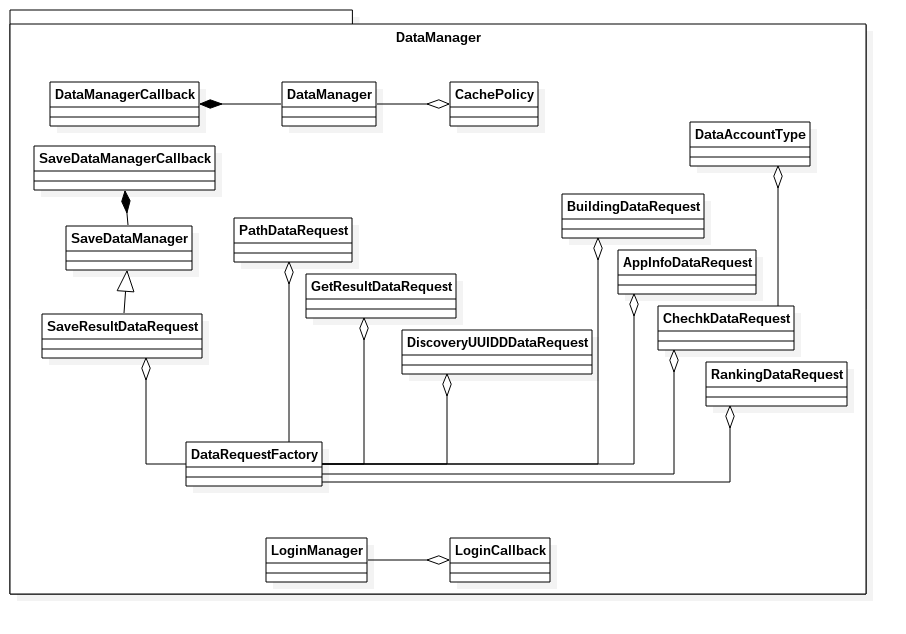
\includegraphics[scale=0.45]{img/package/png/client--datamanager--min.png}
	\caption{Schema sintetico package client::data::datamanager}
\end{figure}
\begin{figure}[h!]
	\centering
	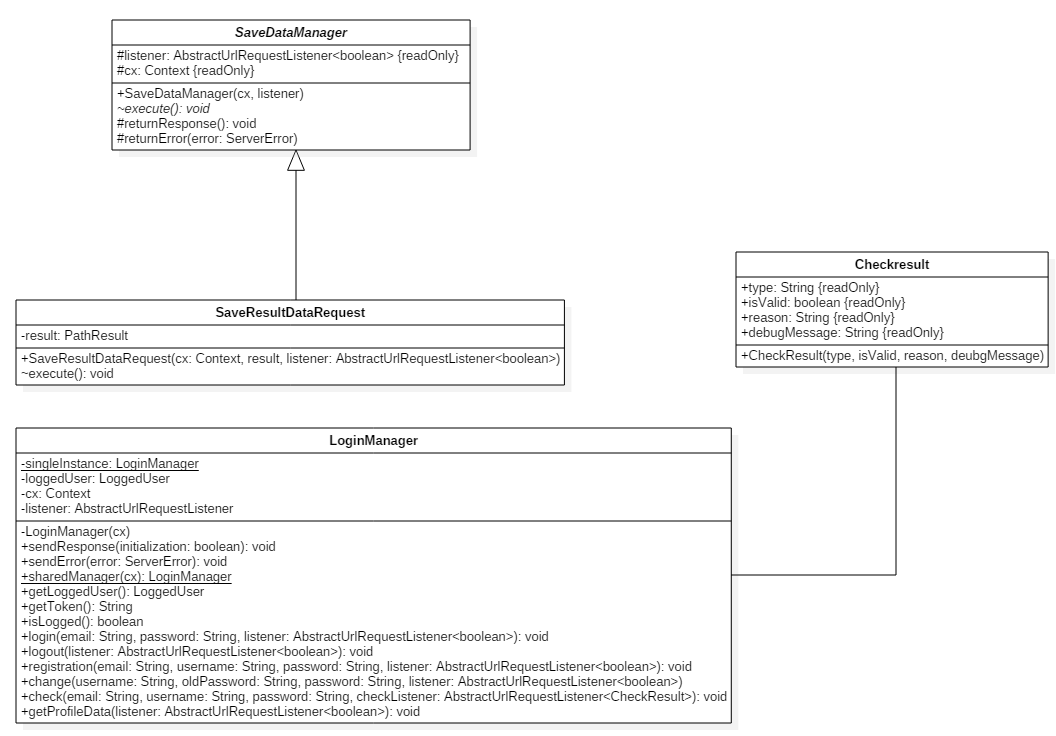
\includegraphics[scale=0.5]{img/package/png/client--datamanager1.png}
	\caption{Prima parte schema package client::data::datamanager}
\end{figure}
\begin{figure}[h!]
	\centering
	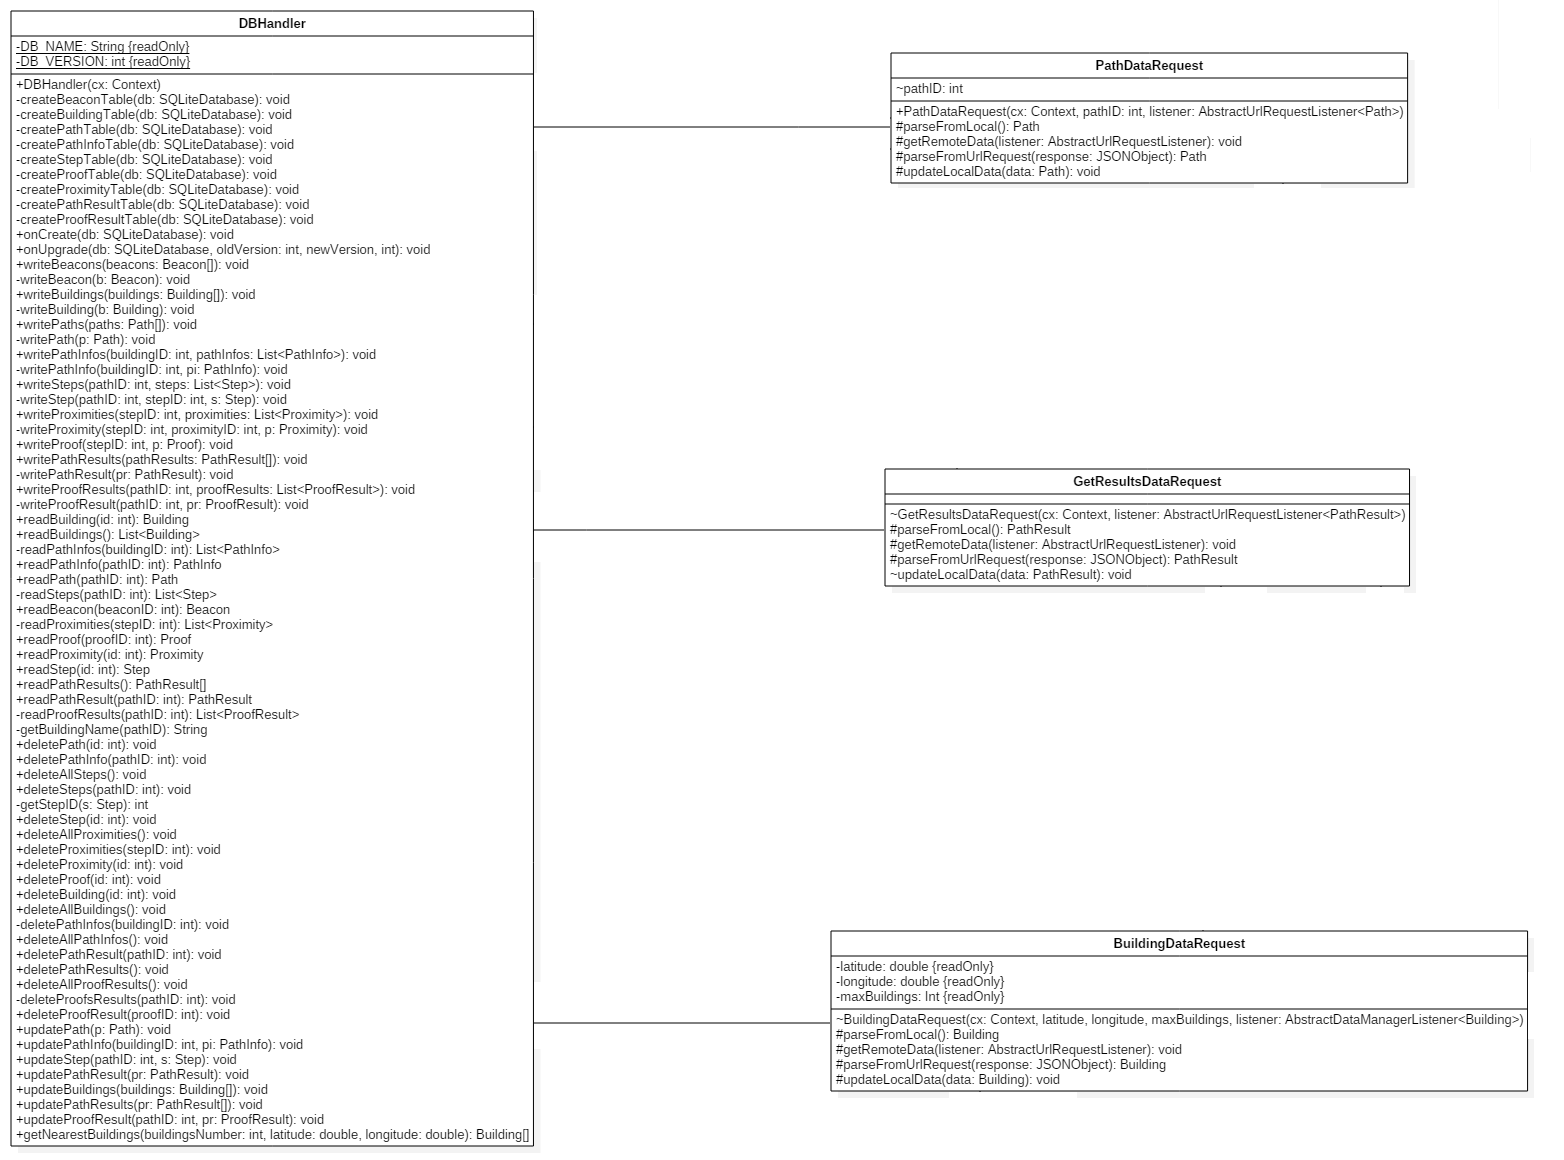
\includegraphics[scale=0.4]{img/package/png/client--datamanager2.png}
	\caption{Seconda parte schema package client::data::datamanager}
\end{figure}
\begin{figure}[h!]
	\centering
	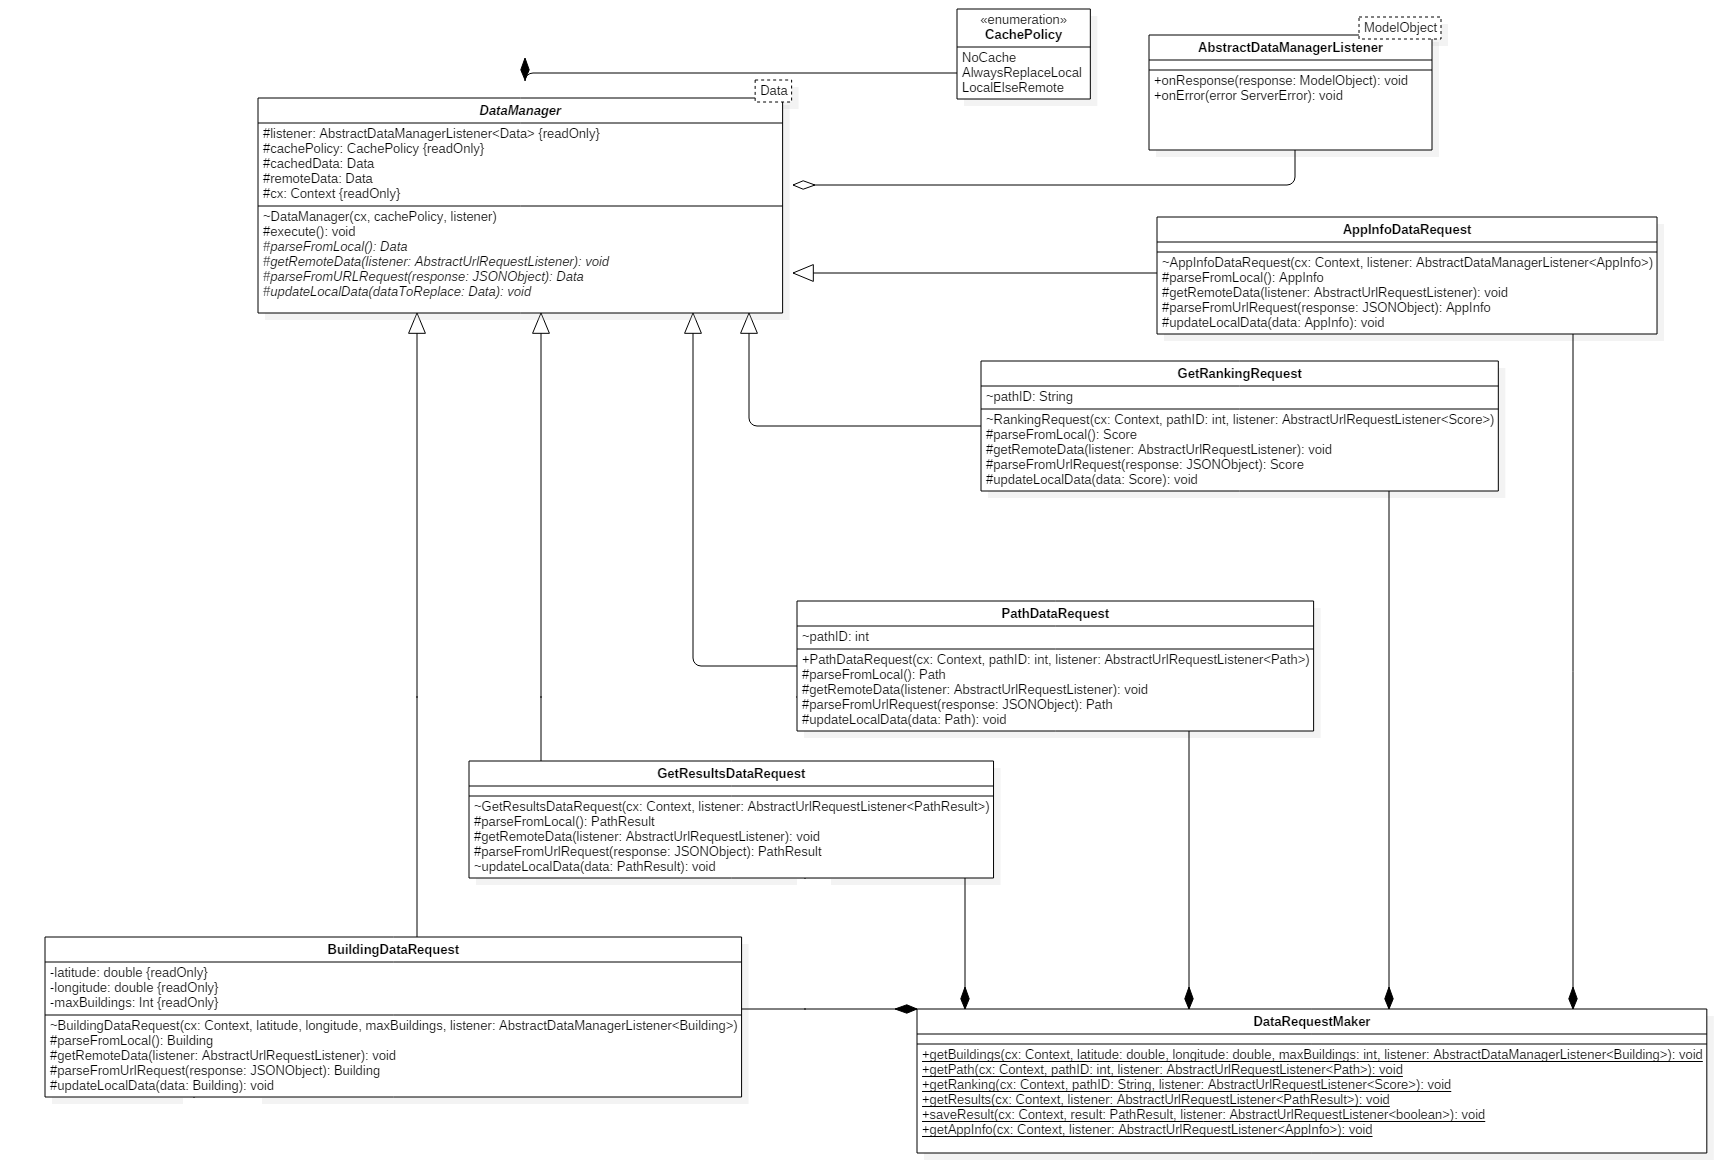
\includegraphics[scale=0.35]{img/package/png/client--datamanager3.png}
	\caption{Terza parte schema package client::data::datamanager}
\end{figure}
\compDescrizione{componente che gestisce i dati in locale}
\compPadre{data}
\begin{compClassi} \\ 
\begin{classe}{CLIPS::client::data::datamanager::/textit{SaveDataManager}}
\classeDescrizione{classe astratta per il salvataggio di dati nel server}
\classeUtilizzo{permette di effettuare il salvataggio dei dati nel server}
\begin{classeRelazioni}
\classeRelazione{CLIPS::client::data::datamanager}{AbstractDataManagerListener}{interfaccia che definisce la struttura del listener astratto usato nel package datamanager}\classeRelazione{CLIPS::client::data::urlrequest}{ServerError}{classe che rappresenta l'errore che il client riceve quando la richiesta al server non ha successo}\end{classeRelazioni}
\end{classe}
\begin{classe}{CLIPS::client::data::datamanager::AbstractDataManagerListener}
\classeDescrizione{interfaccia che definisce la struttura del listener astratto usato nel package datamanager}
\classeUtilizzo{permette alle classi che interagiscono con il datamanager di definire un proprio listener concreto da poter usare per ottenere le informazioni richieste}
\begin{classeRelazioni}
\classeRelazione{CLIPS::client::data::urlrequest}{ServerError}{classe che rappresenta l'errore che il client riceve quando la richiesta al server non ha successo}\end{classeRelazioni}
\end{classe}\begin{classe}{CLIPS::client::data::datamanager::AppInfoDataRequest}
\classeDescrizione{classe concreta che gestisce le richieste dei dati sulle info dell'app}
\classeUtilizzo{permette di ottenere i dati riguardanti le informazioni generali dell'app}
\begin{classeRelazioni}
\classeRelazione{CLIPS::client::data::datamanager}{AbstractDataManagerListener}{interfaccia che definisce la struttura del listener astratto usato nel package datamanager}\classeRelazione{CLIPS::client::data::urlrequest}{AbstractUrlRequestListener}{interfaccia che definisce la struttura del listener astratto usato nel package urlrequest}\classeRelazione{CLIPS::client::data::urlrequest}{AbstractUrlRequestListener}{interfaccia che definisce la struttura del listener astratto usato nel package urlrequest}\classeRelazione{CLIPS::client::data}{AppInfo}{classe per la rappresentazione delle informazioni dell'applicazione}\classeRelazione{CLIPS::client::data::urlrequest}{RequestMaker}{classe per la costruzione e l'invio di richieste al server, funziona come un'interfaccia dell'urlrequest per il resto dell'applicazione e quindi regola l'interazione con il package}\classeRelazione{CLIPS::client::data::urlrequest}{ServerError}{classe che rappresenta l'errore che il client riceve quando la richiesta al server non ha successo}\end{classeRelazioni}
\end{classe}\begin{classe}{CLIPS::client::data::datamanager::BuildingsDataRequest}
\classeDescrizione{classe concreta che gestisce le richieste al server per ottenere i dati riguardanti gli edifici abilitati ad utilizzare l'applicazione}
\classeUtilizzo{permette di ottenere i dati sugli edifici}
\begin{classeRelazioni}
\classeRelazione{CLIPS::client::data::datamanager}{AbstractDataManagerListener}{interfaccia che definisce la struttura del listener astratto usato nel package datamanager}\classeRelazione{CLIPS::client::data::urlrequest}{AbstractUrlRequestListener}{interfaccia che definisce la struttura del listener astratto usato nel package urlrequest}\classeRelazione{CLIPS::client::data}{Building}{classe che rappresenta un edificio}\classeRelazione{CLIPS::server::urlrequesthandler}{DBHandler}{classe che si occupa di gestire il DB e di ritornare un oggetto configurato della libreria knex}\classeRelazione{CLIPS::client::data}{PathInfo}{classe che si occupa di salvare in locale le informazioni generali di un percorso}\classeRelazione{CLIPS::client::data::urlrequest}{RequestMaker}{classe per la costruzione e l'invio di richieste al server, funziona come un'interfaccia dell'urlrequest per il resto dell'applicazione e quindi regola l'interazione con il package}\classeRelazione{CLIPS::client::data::urlrequest}{ServerError}{classe che rappresenta l'errore che il client riceve quando la richiesta al server non ha successo}\end{classeRelazioni}
\end{classe}\begin{classe}{CLIPS::client::data::datamanager::CheckResult}
\classeDescrizione{classe che contiene il risultato del check per il dato specificato}
\classeUtilizzo{contiene tutte le informazioni sul dato controllato dal server, ovvero se è valido e il messaggio d'errore quando ne viene rilevato uno}
\begin{classeRelazioni}
\classeRelazione{CLIPS::client::data::datamanager}{AbstractDataManagerListener}{interfaccia che definisce la struttura del listener astratto usato nel package datamanager}\classeRelazione{CLIPS::client::data::urlrequest}{AbstractUrlRequestListener}{interfaccia che definisce la struttura del listener astratto usato nel package urlrequest}\classeRelazione{CLIPS::client::data::urlrequest}{ServerError}{classe che rappresenta l'errore che il client riceve quando la richiesta al server non ha successo}\end{classeRelazioni}
\end{classe}\begin{classe}{CLIPS::client::data::datamanager::DataRequestMaker}
\classeDescrizione{classe che effettua le operazioni di ricerca e salvataggio dei dati}
\classeUtilizzo{permette di effettuare operazioni di salvataggio dei dati nel server e di ricerca dei dati, richiedendoli al server o cercandoli in locale}
\begin{classeRelazioni}
\classeRelazione{CLIPS::client::data::datamanager}{AbstractDataManagerListener}{interfaccia che definisce la struttura del listener astratto usato nel package datamanager}\classeRelazione{CLIPS::client::data}{AppInfo}{classe per la rappresentazione delle informazioni dell'applicazione}\classeRelazione{CLIPS::client::data::datamanager}{AppInfoDataRequest}{classe concreta che gestisce le richieste dei dati sulle info dell'app}\classeRelazione{CLIPS::client::data}{Building}{classe che rappresenta un edificio}\classeRelazione{CLIPS::client::data::datamanager}{BuildingsDataRequest}{classe concreta che gestisce le richieste dei dati sugli edifici}\classeRelazione{CLIPS::client::data::datamanager}{GetRankingDataRequest}{classe concreta che gestisce le richieste dei dati della classifica}\classeRelazione{CLIPS::client::data::datamanager}{GetResultsDataRequest}{classe concreta che gestisce le richieste dei dati dei risultati}\classeRelazione{CLIPS::client::data}{Path}{classe che si occupa di salvare in locale i dati riguardanti un percorso}\classeRelazione{CLIPS::client::data::datamanager}{PathDataRequest}{classe concreta che gestisce le richieste dei dati sui percorsi}\classeRelazione{CLIPS::client::data}{PathResult}{classe che rappresenta i risultati di un percorso}\classeRelazione{CLIPS::client::data::datamanager}{SaveResultDataRequest}{classe concreta che effettua le richieste per salvare il risultato del percorso appena concluso}\classeRelazione{CLIPS::client::data}{Score}{classe che rappresenta il risultato nella classifica dell'utente}\end{classeRelazioni}
\end{classe}\begin{classe}{CLIPS::client::data::datamanager::DBHandler}
\classeDescrizione{classe che si occupa della gestione del database locale}
\classeUtilizzo{utilizzando questa classe è possibile interagire con il database locale per ottenere e salvare i dati desiderati}
\end{classe}\begin{classe}{CLIPS::client::data::datamanager::GetRankingDataRequest}
\classeDescrizione{classe concreta che gestisce le richieste dei dati della classifica}
\classeUtilizzo{permette di ottenere i dati della classifica}

\begin{classeRelazioni}
\classeRelazione{CLIPS::client::data::datamanager}{AbstractDataManagerListener}{interfaccia che definisce la struttura del listener astratto usato nel package datamanager}\classeRelazione{CLIPS::client::data::urlrequest}{AbstractUrlRequestListener}{interfaccia che definisce la struttura del listener astratto usato nel package urlrequest}\classeRelazione{CLIPS::client::data::urlrequest}{RequestMaker}{classe per la costruzione e l'invio di richieste al server, funziona come un'interfaccia dell'urlrequest per il resto dell'applicazione e quindi regola l'interazione con il package}\classeRelazione{CLIPS::client::data}{Score}{classe che rappresenta il risultato nella classifica dell'utente}\classeRelazione{CLIPS::client::data::urlrequest}{ServerError}{classe che rappresenta l'errore che il client riceve quando la richiesta al server non ha successo}\end{classeRelazioni}
\end{classe}\begin{classe}{CLIPS::client::data::datamanager::GetResultsDataRequest}
\classeDescrizione{classe concreta che gestisce le richieste dei dati dei risultati delle prove}
\classeUtilizzo{permette di ottenere i dati dei risultati}
\begin{classeRelazioni}
\classeRelazione{CLIPS::client::data::datamanager}{AbstractDataManagerListener}{interfaccia che definisce la struttura del listener astratto usato nel package datamanager}\classeRelazione{CLIPS::client::data::urlrequest}{AbstractUrlRequestListener}{interfaccia che definisce la struttura del listener astratto usato nel package urlrequest}\classeRelazione{CLIPS::server::urlrequesthandler}{DBHandler}{classe che si occupa di gestire il DB e di ritornare un oggetto configurato della libreria knex}\classeRelazione{CLIPS::client::data}{PathResult}{classe che rappresenta i risultati di un percorso}\classeRelazione{CLIPS::client::data}{ProofResult}{classe che rappresenta il risultato di una prova}\classeRelazione{CLIPS::client::data::urlrequest}{RequestMaker}{classe per la costruzione e l'invio di richieste al server, funziona come un'interfaccia dell'urlrequest per il resto dell'applicazione e regola l'interazione con il package}\classeRelazione{CLIPS::client::data::urlrequest}{ServerError}{classe che rappresenta l'errore che il client riceve quando la richiesta al server non ha successo}\end{classeRelazioni}
\end{classe}\begin{classe}{CLIPS::client::data::datamanager::LoginManager}
\classeDescrizione{classe che gestisce le operazioni del profilo dell'utente}
\classeUtilizzo{permette di effettuare il login, il logout, la registrazione, il check dei dati inseriti, l'aggiornamento dei dati salvati in locale e la modifica dei dati del profilo}
\begin{classeRelazioni}
\classeRelazione{CLIPS::client::data::datamanager}{AbstractDataManagerListener}{interfaccia che definisce la struttura del listener astratto usato nel package datamanager}\classeRelazione{CLIPS::client::data::urlrequest}{AbstractUrlRequestListener}{interfaccia che definisce la struttura del listener astratto usato nel package urlrequest}\classeRelazione{CLIPS::client::data::datamanager}{CheckResult}{classe che contiene il risultato del check per il dato specificato}\classeRelazione{CLIPS::client::data}{LoggedUser}{classe che si occupa di memorizzare in locale i dati dell'utente loggato}\classeRelazione{CLIPS::client::data::urlrequest}{RequestMaker}{classe per la costruzione e l'invio di richieste al server, funziona come un'interfaccia dell'urlrequest per il resto dell'applicazione e regola l'interazione con il package}\classeRelazione{CLIPS::client::data::urlrequest}{ServerError}{classe che rappresenta l'errore che il client riceve quando la richiesta al server non ha successo}\end{classeRelazioni}
\end{classe}\begin{classe}{CLIPS::client::data::datamanager::PathDataRequest}
\classeDescrizione{classe concreta che gestisce le richieste dei dati sui percorsi di un edificio}
\classeUtilizzo{permette di ottenere i dati sui percorsi}
\begin{classeRelazioni}
\classeRelazione{CLIPS::client::data::datamanager}{AbstractDataManagerListener}{interfaccia che definisce la struttura del listener astratto usato nel package datamanager}\classeRelazione{CLIPS::client::data::urlrequest}{AbstractUrlRequestListener}{interfaccia che definisce la struttura del listener astratto usato nel package urlrequest}\classeRelazione{CLIPS::client::data}{Beacon}{classe che rappresenta un beacon in locale}\classeRelazione{CLIPS::server::urlrequesthandler}{DBHandler}{classe che si occupa di gestire il DB e di ritornare un oggetto configurato della libreria knex}\classeRelazione{CLIPS::client::data}{Path}{classe che si occupa di salvare in locale i dati riguardanti un percorso}\classeRelazione{CLIPS::client::data}{Proof}{classe che rappresenta una prova del percorso}\classeRelazione{CLIPS::client::data}{Proximity}{classe che rappresenta in locale un beacon indicato alla segnalazione della distanza dalla prossima prova}\classeRelazione{CLIPS::client::data::urlrequest}{ServerError}{classe che rappresenta l'errore che il client riceve quando la richiesta al server non ha successo}\classeRelazione{CLIPS::client::data::urlrequest}{ServerError}{classe che rappresenta l'errore che il client riceve quando la richiesta al server non ha successo}\classeRelazione{CLIPS::client::data}{Step}{classe che rappresenta in locale lo spostamento da una prova a quella successiva}\end{classeRelazioni}
\end{classe}\begin{classe}{CLIPS::client::data::datamanager::SaveResultDataRequest}
\classeDescrizione{classe concreta che effettua le richieste per salvare il risultato del percorso appena concluso}
\classeUtilizzo{permette di salvare in remoto il risultato del percorso appena svolto}
\begin{classeRelazioni}
\classeRelazione{CLIPS::client::data::datamanager}{AbstractDataManagerListener}{interfaccia che definisce la struttura del listener astratto usato nel package datamanager}\classeRelazione{CLIPS::client::data::urlrequest}{AbstractUrlRequestListener}{interfaccia che definisce la struttura del listener astratto usato nel package urlrequest}\classeRelazione{CLIPS::client::data}{PathResult}{classe che rappresenta i risultati di un percorso}\classeRelazione{CLIPS::client::data::urlrequest}{RequestMaker}{classe per la costruzione e l'invio di richieste al server, funziona come un'interfaccia dell'urlrequest per il resto dell'applicazione e quindi regola l'interazione con il package}\classeRelazione{CLIPS::client::data::urlrequest}{ServerError}{classe che rappresenta l'errore che il client riceve quando la richiesta al server non ha successo}\classeRelazione{CLIPS::client::data::urlrequest}{ServerError}{classe che rappresenta l'errore che il client riceve quando la richiesta al server non ha successo}\end{classeRelazioni}
\end{classe}\end{compClassi}
\end{componente}
\begin{componente}{CLIPS::client::data::urlrequest}
\begin{figure}[h!]
	\centering
	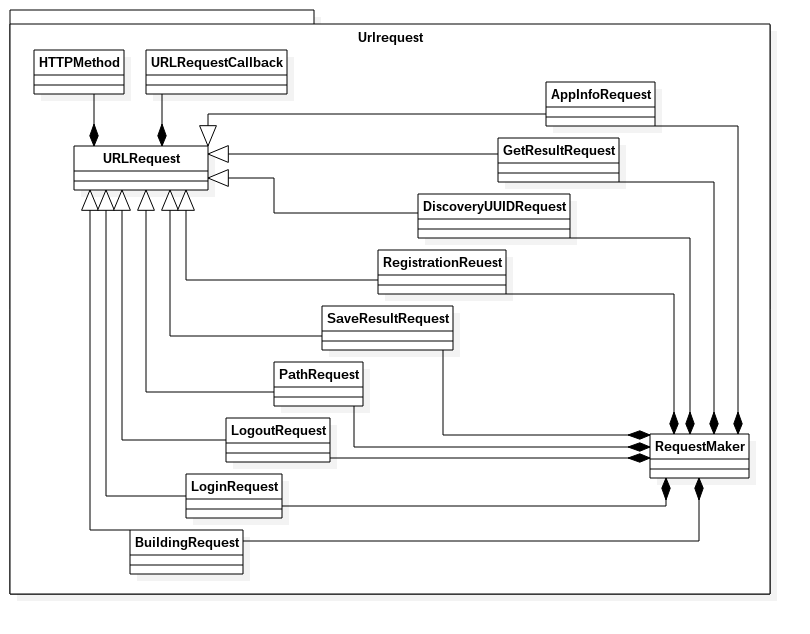
\includegraphics[scale=0.45]{img/package/png/client--urlrequest--min.png}
	\caption{Schema sintetico package client::data::urlrequest}
\end{figure}
\begin{figure}[h!]
	\centering
	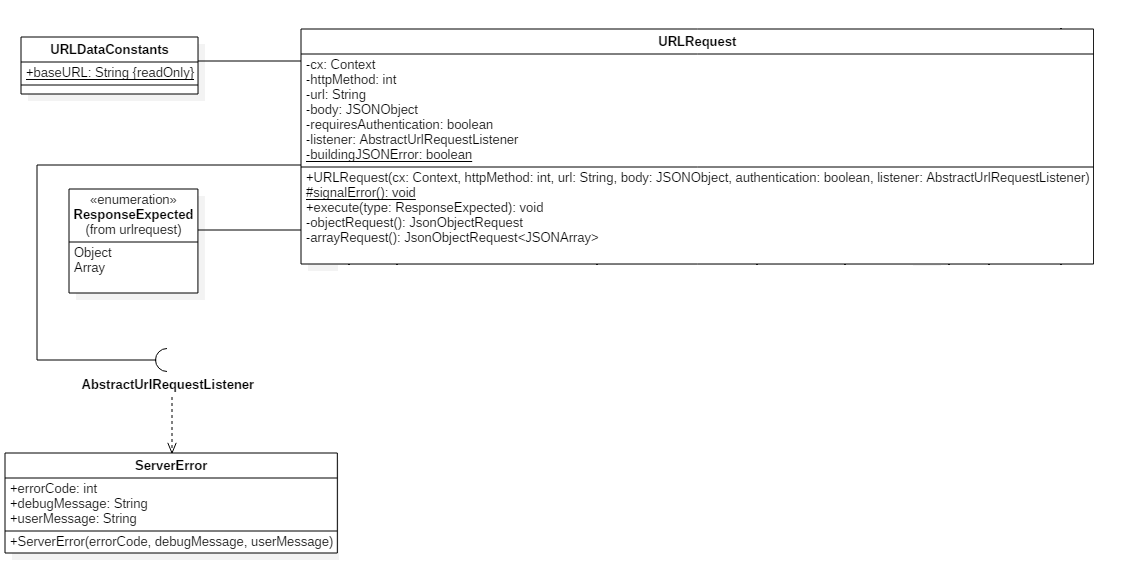
\includegraphics[scale=0.5]{img/package/png/client--urlrequest1.png}
	\caption{Prima parte schema package client::data::urlrequest}
\end{figure}
\begin{figure}[h!]
	\centering
	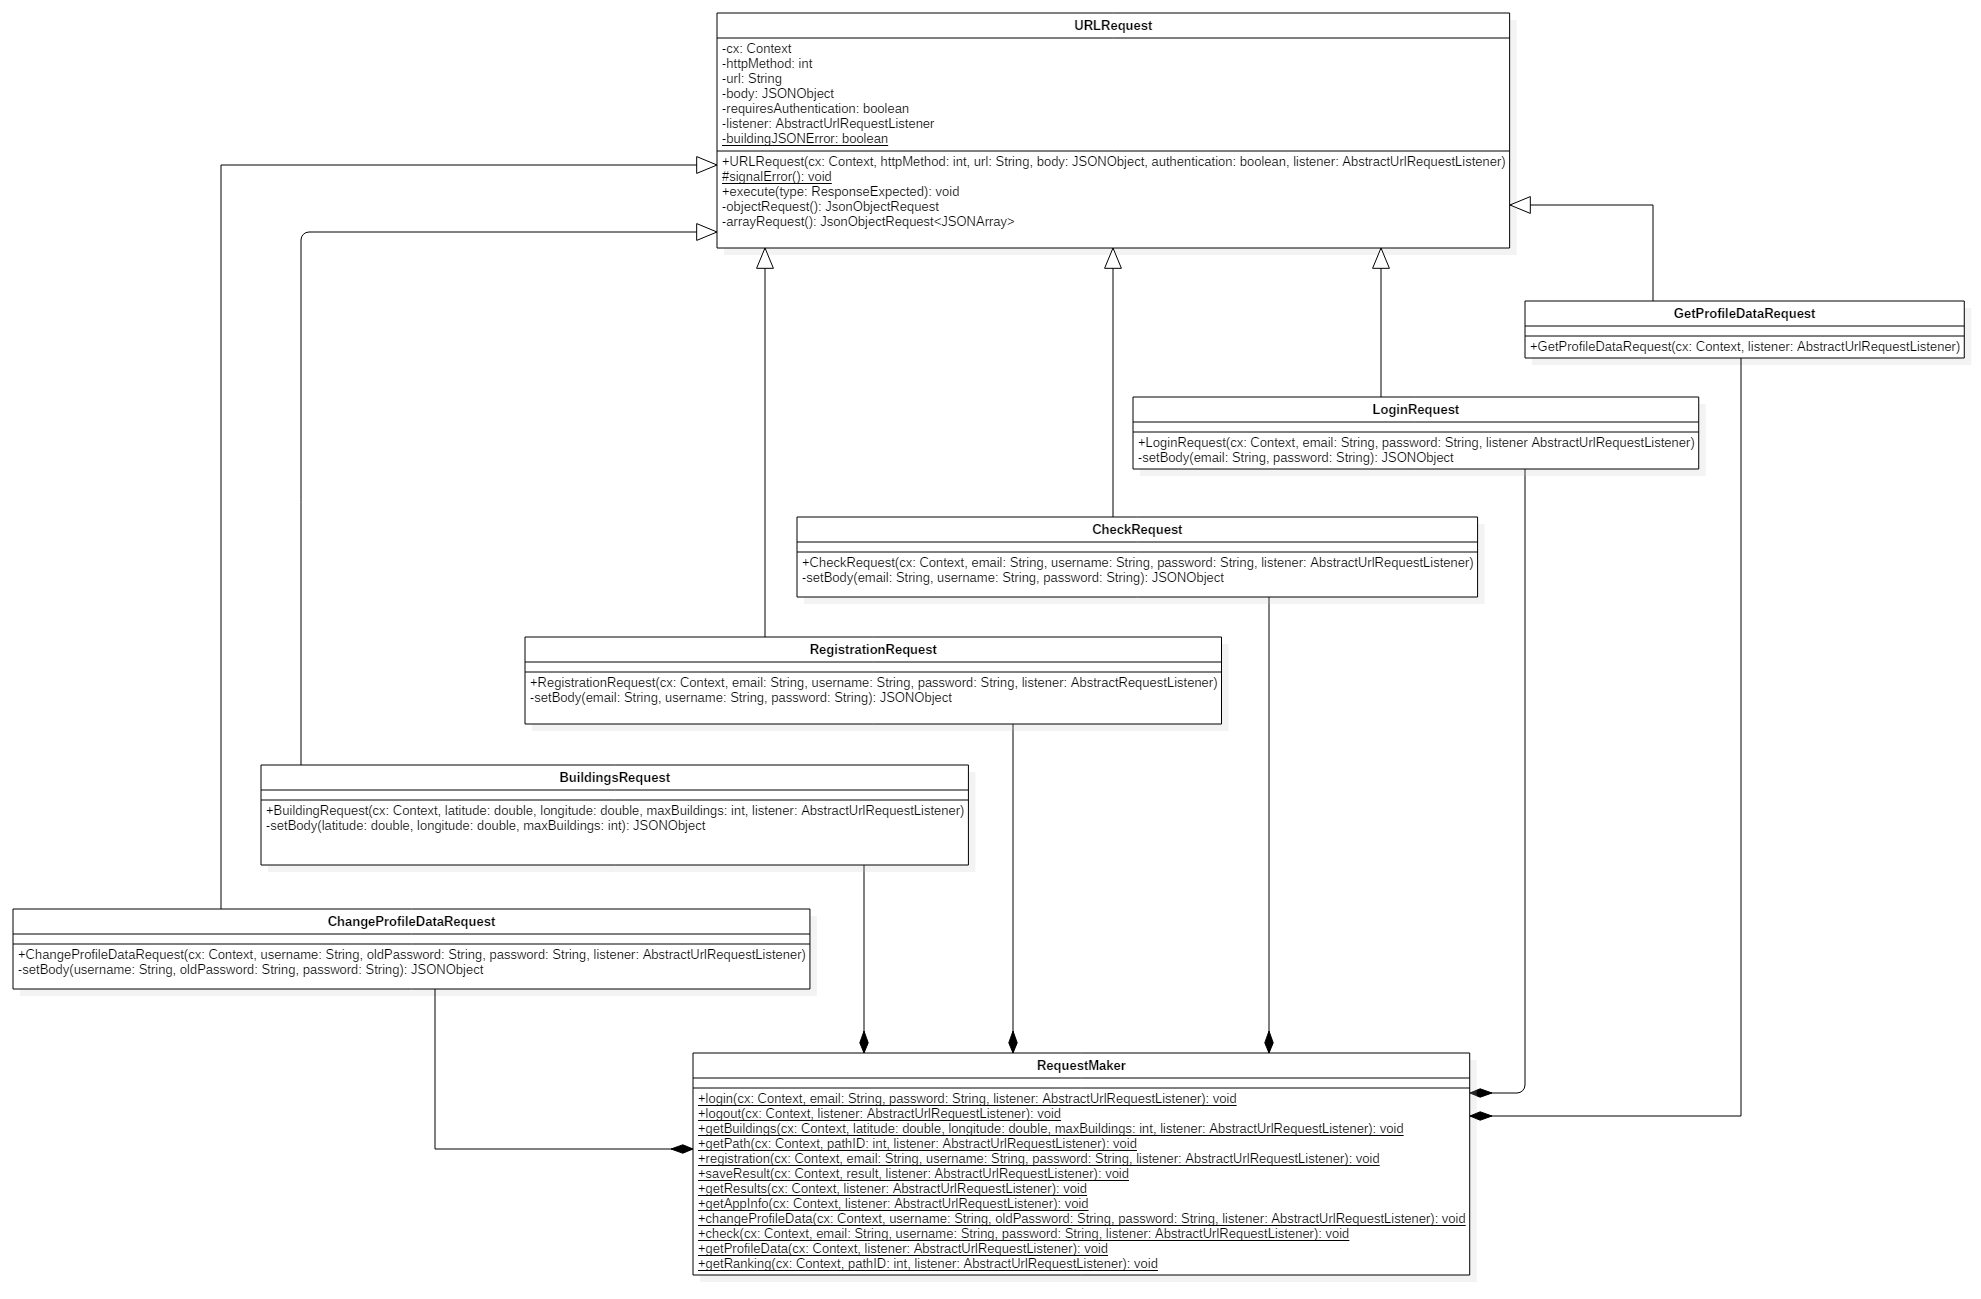
\includegraphics[scale=0.30]{img/package/png/client--urlrequest2.png}
	\caption{Seconda parte schema package client::data::urlrequest}
\end{figure}
\begin{figure}[h!]
	\centering
	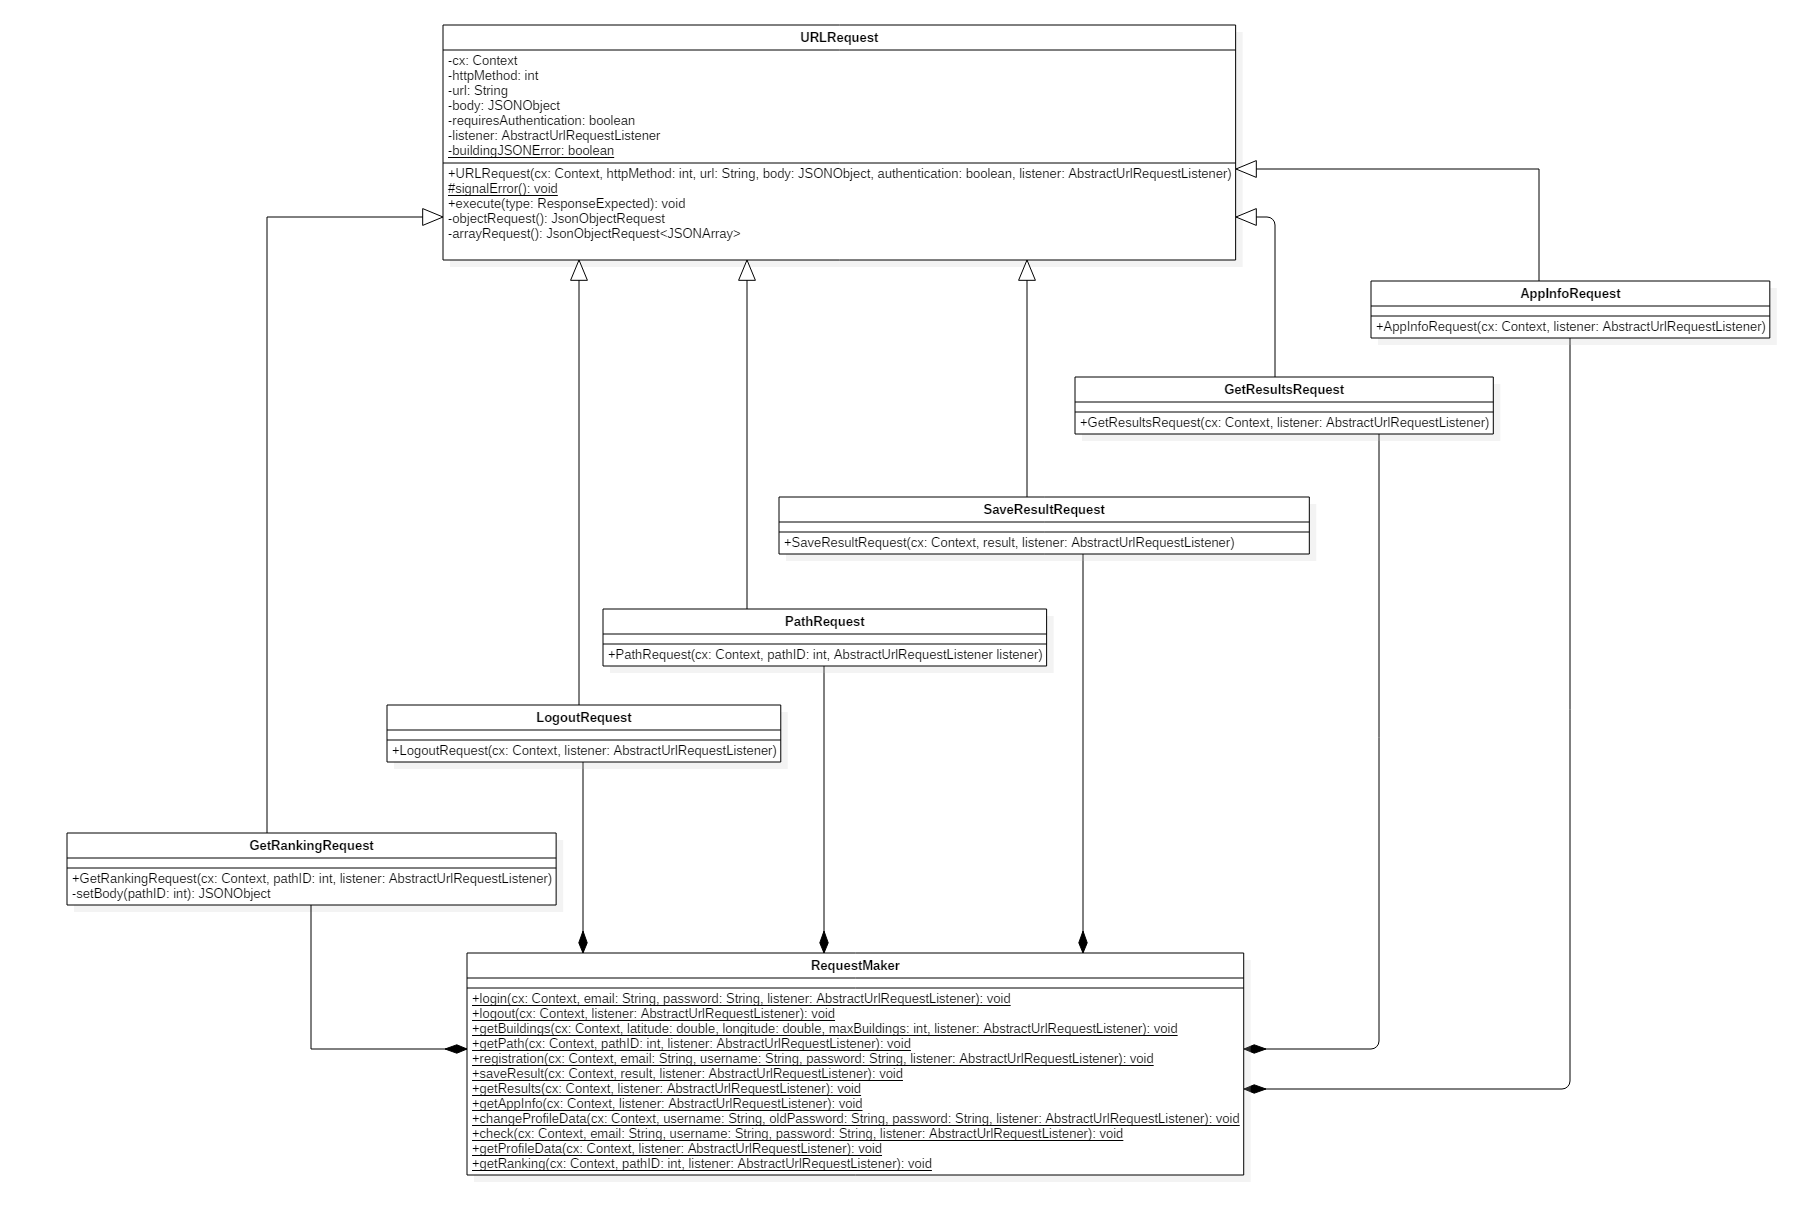
\includegraphics[scale=0.35]{img/package/png/client--urlrequest3.png}
	\caption{Terza parte schema package client::data::urlrequest}
\end{figure}
\compDescrizione{componente che si occupa di effettuare le richieste al server}
\compPadre{data}
\begin{compClassi} \\ 
\begin{classe}{CLIPS::client::data::urlrequest::AbstractUrlRequestListener}
\classeDescrizione{interfaccia che definisce la struttura del listener astratto usato nel package urlrequest}
\classeUtilizzo{permette alle classi che interagiscono con l'urlrequest di definire un proprio listener concreto da poter usare per le chiamate al server}
\begin{classeRelazioni}
\classeRelazione{CLIPS::client::data::urlrequest}{ServerError}{classe che rappresenta l'errore che il client riceve quando la richiesta al server non ha successo}\end{classeRelazioni}
\end{classe}\begin{classe}{CLIPS::client::data::urlrequest::AppInfoRequest}
\classeDescrizione{classe per la richiesta al server di dati sulle info dell'app, tra cui lo UUID dei beacon usati per l'applicazione e le informazioni sull'applicazione}
\classeUtilizzo{permette di effettuare una richiesta al server di dati sulle info dell'app}
\begin{classeRelazioni}
\classeRelazione{CLIPS::client::data::urlrequest}{AbstractUrlRequestListener}{interfaccia che definisce la struttura del listener astratto usato nel package urlrequest}\classeRelazione{CLIPS::client::data::urlrequest}{URLDataConstants}{classe che contiene i dati per effettuare le richieste al server che potrebbero variare nel tempo}\end{classeRelazioni}
\end{classe}\begin{classe}{CLIPS::client::data::urlrequest::BuildingsRequest}
\classeDescrizione{classe per la richiesta di dati sugli edifici}
\classeUtilizzo{permette di effettuare una richiesta al server di dati sugli edifici}
\begin{classeRelazioni}
\classeRelazione{CLIPS::client::data::urlrequest}{AbstractUrlRequestListener}{interfaccia che definisce la struttura del listener astratto usato nel package urlrequest}\classeRelazione{CLIPS::client::data::urlrequest}{URLDataConstants}{classe che contiene i dati per effettuare le richieste al server che potrebbero variare nel tempo}\end{classeRelazioni}
\end{classe}\begin{classe}{CLIPS::client::data::urlrequest::ChangeProfileDataRequest}
\classeDescrizione{classe per la richiesta al server di cambiare i dati dell'utente}
\classeUtilizzo{permette di inviare la richiesta al server di cambiare i dati dell'utente, in particolare possono essere modificati solo lo username e la password}
\begin{classeRelazioni}
\classeRelazione{CLIPS::client::data::urlrequest}{AbstractUrlRequestListener}{interfaccia che definisce la struttura del listener astratto usato nel package urlrequest}\classeRelazione{CLIPS::client::data::urlrequest}{URLDataConstants}{classe che contiene i dati per effettuare le richieste al server che potrebbero variare nel tempo}\end{classeRelazioni}
\end{classe}\begin{classe}{CLIPS::client::data::urlrequest::CheckRequest}
\classeDescrizione{classe per la richiesta al server del controllo dei dati inseriti dall'utente}
\classeUtilizzo{permette di inviare la richiesta al server per controllare se l'email, lo username o la password sono corretti}
\begin{classeRelazioni}
\classeRelazione{CLIPS::client::data::urlrequest}{AbstractUrlRequestListener}{interfaccia che definisce la struttura del listener astratto usato nel package urlrequest}\classeRelazione{CLIPS::client::data::urlrequest}{URLDataConstants}{classe che contiene i dati per effettuare le richieste al server che potrebbero variare nel tempo}\end{classeRelazioni}
\end{classe}\begin{classe}{CLIPS::client::data::urlrequest::ForgotPasswordRequest}
\classeDescrizione{Classe che effettua la richiesta di cambiare la password dimenticata dell'utente}
\classeUtilizzo{Quando l'utente non ricorda la password può usare questa chiamata per ottenerne una generata casualmente dopo aver inserito l'indirizzo email dell'account da cambiare}
\begin{classeRelazioni}
\classeRelazione{CLIPS::client::data::urlrequest}{URLDataConstants}{classe che contiene i dati per effettuare le richieste al server che potrebbero variare nel tempo}\classeRelazione{CLIPS::client::data::urlrequest}{URLRequest}{classe che si occupa delle richieste da inviare al server, fornisce un'implementazione delle richieste in base ai dati forniti alle sue classi derivate}\end{classeRelazioni}
\end{classe}\begin{classe}{CLIPS::client::data::urlrequest::GetProfileDataRequest}
\classeDescrizione{classe per la richiesta al server di aggiornare in locale i dati dell'utente}
\classeUtilizzo{permette di inviare la richiesta al server per aggiornare l'email e lo username dell'utente nel caso non fossero uguali a quelli salvati nel server}
\begin{classeRelazioni}
\classeRelazione{CLIPS::client::data::urlrequest}{AbstractUrlRequestListener}{interfaccia che definisce la struttura del listener astratto usato nel package urlrequest}\classeRelazione{CLIPS::client::data::urlrequest}{URLDataConstants}{classe che contiene i dati per effettuare le richieste al server che potrebbero variare nel tempo}\end{classeRelazioni}
\end{classe}\begin{classe}{CLIPS::client::data::urlrequest::GetRankingRequest}
\classeDescrizione{classe per la richiesta al server dei dati sulla classifica di un determinato percorso}
\classeUtilizzo{permette di inviare la richiesta al server per ottenere i dati sulla classifica del percorso selezionato}
\begin{classeRelazioni}
\classeRelazione{CLIPS::client::data::urlrequest}{AbstractUrlRequestListener}{interfaccia che definisce la struttura del listener astratto usato nel package urlrequest}\classeRelazione{CLIPS::client::data::urlrequest}{URLDataConstants}{classe che contiene i dati per effettuare le richieste al server che potrebbero variare nel tempo}\end{classeRelazioni}
\end{classe}\begin{classe}{CLIPS::client::data::urlrequest::GetResultsRequest}
\classeDescrizione{classe per la richiesta al server dei risultati salvati dall'utente in precedenza}
\classeUtilizzo{permette di effettuare la richiesta al server dei risultati salvati dall'utente in precedenza}
\begin{classeRelazioni}
\classeRelazione{CLIPS::client::data::urlrequest}{AbstractUrlRequestListener}{interfaccia che definisce la struttura del listener astratto usato nel package urlrequest}\classeRelazione{CLIPS::client::data::urlrequest}{URLDataConstants}{classe che contiene i dati per effettuare le richieste al server che potrebbero variare nel tempo}\end{classeRelazioni}
\end{classe}\begin{classe}{CLIPS::client::data::urlrequest::LoginRequest}
\classeDescrizione{classe per la richiesta di login al server}
\classeUtilizzo{permette di effettuare una richiesta di login al server}
\begin{classeRelazioni}
\classeRelazione{CLIPS::client::data::urlrequest}{AbstractUrlRequestListener}{interfaccia che definisce la struttura del listener astratto usato nel package urlrequest}\classeRelazione{CLIPS::client::data::urlrequest}{URLDataConstants}{classe che contiene i dati per effettuare le richieste al server che potrebbero variare nel tempo}\end{classeRelazioni}
\end{classe}\begin{classe}{CLIPS::client::data::urlrequest::LogoutRequest}
\classeDescrizione{classe per la richiesta di logout al server}
\classeUtilizzo{permette di effettuare una richiesta di logout al server}
\begin{classeRelazioni}
\classeRelazione{CLIPS::client::data::urlrequest}{AbstractUrlRequestListener}{interfaccia che definisce la struttura del listener astratto usato nel package urlrequest}\classeRelazione{CLIPS::client::data::urlrequest}{URLDataConstants}{classe che contiene i dati per effettuare le richieste al server che potrebbero variare nel tempo}\end{classeRelazioni}
\end{classe}\begin{classe}{CLIPS::client::data::urlrequest::PathRequest}
\classeDescrizione{classe per la richiesta al server dei dati sul percorso selezionato, in particolare fornisce tutte le informazioni necessarie per poter svolgere il percorso}
\classeUtilizzo{permette di richiedere al server i dati sul percorso selezionato}
\begin{classeRelazioni}
\classeRelazione{CLIPS::client::data::urlrequest}{AbstractUrlRequestListener}{interfaccia che definisce la struttura del listener astratto usato nel package urlrequest}\classeRelazione{CLIPS::client::data::urlrequest}{URLDataConstants}{classe che contiene i dati per effettuare le richieste al server che potrebbero variare nel tempo}\end{classeRelazioni}
\end{classe}\begin{classe}{CLIPS::client::data::urlrequest::RegistrationRequest}
\classeDescrizione{classe per la richiesta di registrazione al server}
\classeUtilizzo{permette di effettuare una richiesta di registrazione al server}
\begin{classeRelazioni}
\classeRelazione{CLIPS::client::data::urlrequest}{AbstractUrlRequestListener}{interfaccia che definisce la struttura del listener astratto usato nel package urlrequest}\classeRelazione{CLIPS::client::data::urlrequest}{URLDataConstants}{classe che contiene i dati per effettuare le richieste al server che potrebbero variare nel tempo}\end{classeRelazioni}
\end{classe}\begin{classe}{CLIPS::client::data::urlrequest::RequestMaker}
\classeDescrizione{classe per la costruzione e l'invio di richieste al server, funziona come un'interfaccia dell'urlrequest per il resto dell'applicazione e quindi regola l'interazione con il package}
\classeUtilizzo{permette la costruzione e l'invio di richieste al server}
\begin{classeRelazioni}
\classeRelazione{CLIPS::client::data::urlrequest}{AbstractUrlRequestListener}{interfaccia che definisce la struttura del listener astratto usato nel package urlrequest}\classeRelazione{CLIPS::client::data::urlrequest}{AppInfoRequest}{classe per la richiesta al server di dati sulle info dell'app, tra cui lo UUID dei beacon usati per l'applicazione e le informazioni sull'applicazione}\classeRelazione{CLIPS::client::data::urlrequest}{BuildingsRequest}{classe per la richiesta di dati sugli edifici}\classeRelazione{CLIPS::client::data::urlrequest}{ChangeProfileDataRequest}{classe per la richiesta al server di cambiare i dati dell'utente}\classeRelazione{CLIPS::client::data::urlrequest}{CheckRequest}{classe per la richiesta al server del controllo dei dati inseriti dall'utente}\classeRelazione{CLIPS::client::data::urlrequest}{GetProfileDataRequest}{classe per la richiesta al server di aggiornare in locale i dati dell'utente}\classeRelazione{CLIPS::client::data::urlrequest}{GetRankingRequest}{classe per la richiesta al server dei dati sulla classifica di un determinato percorso}\classeRelazione{CLIPS::client::data::urlrequest}{GetResultsRequest}{classe per la richiesta al server dei risultati salvati dall'utente in precedenza}\classeRelazione{CLIPS::client::data::urlrequest}{LoginRequest}{classe per la richiesta di login al server}\classeRelazione{CLIPS::client::data::urlrequest}{LogoutRequest}{classe per la richiesta di logout al server}\classeRelazione{CLIPS::client::data::urlrequest}{PathRequest}{classe per la richiesta al server dei dati sul percorso selezionato, in particolare fornisce tutte le informazioni necessarie per poter svolgere il percorso}\classeRelazione{CLIPS::client::data}{PathResult}{classe che rappresenta i risultati di un percorso}\classeRelazione{CLIPS::client::data::urlrequest}{RegistrationRequest}{classe per la richiesta di registrazione al server}\classeRelazione{CLIPS::client::data::urlrequest}{SaveResultRequest}{classe per la richiesta al server di salvataggio del risultato del percorso appena finito}\end{classeRelazioni}
\end{classe}\begin{classe}{CLIPS::client::data::urlrequest::SaveResultRequest}
\classeDescrizione{classe per la richiesta al server di salvataggio del risultato del percorso appena finito}
\classeUtilizzo{permette di effettuare una richiesta al server di salvataggio del risultato del percorso appena finito}
\end{classe}\begin{classe}{CLIPS::client::data::urlrequest::ServerError}
\classeDescrizione{classe che rappresenta l'errore che il client riceve quando la richiesta al server non ha successo}
\classeUtilizzo{permette di rappresentare l'errore ricevuto in una forma più semplice da usare nel resto dell'applicazione}
\end{classe}\begin{classe}{CLIPS::client::data::urlrequest::URLDataConstants}
\classeDescrizione{classe che contiene i dati per effettuare le richieste al server che potrebbero variare nel tempo}
\classeUtilizzo{permette di gestire facilmente eventuali cambiamenti futuri dei dati necessari ad effettuare le richieste al server}
\end{classe}\begin{classe}{CLIPS::client::data::urlrequest::URLRequest}
\classeDescrizione{classe che si occupa delle richieste da inviare al server, fornisce un'implementazione delle richieste in base ai dati forniti alle sue classi derivate}
\classeUtilizzo{permette di effettuare tutte le richieste al server necessarie per far funzionare l'applicazione}
\begin{classeRelazioni}
\classeRelazione{CLIPS::client::data::urlrequest}{AbstractUrlRequestListener}{interfaccia che definisce la struttura del listener astratto usato nel package urlrequest}\classeRelazione{CLIPS::client::data::datamanager}{LoginManager}{classe che gestisce le operazioni del profilo dell'utente}\classeRelazione{CLIPS::client::data::urlrequest}{ServerError}{classe che rappresenta l'errore che il client riceve quando la richiesta al server non ha successo}\end{classeRelazioni}
\end{classe}\end{compClassi}
\end{componente}
\begin{componente}{CLIPS::client::pathprogress}
\begin{figure}[h!] 
\centering 
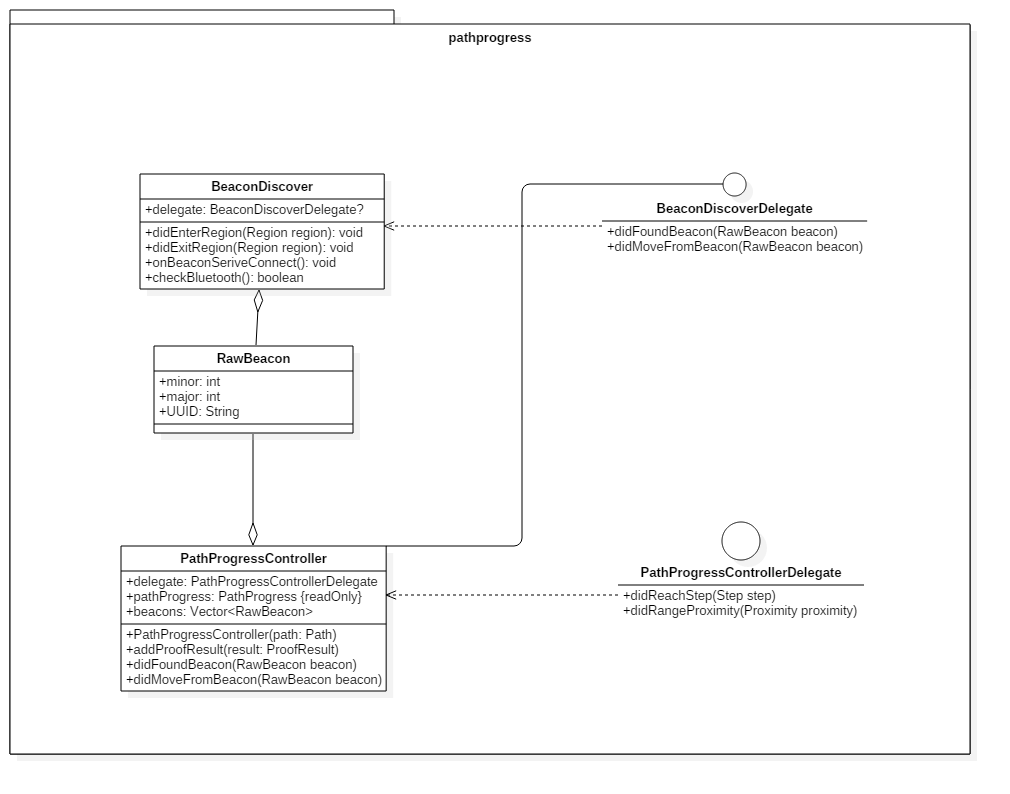
\includegraphics[scale=0.3]{img/package/png/client--pathprogress.png} 
\caption{Schema package client::pathprogress} 
 \end{figure} 
\compDescrizione{componente che gestisce i dati del percorso e salva i risultati ottenuti nelle prove mentre si sta giocando}
\compPadre{client}
\begin{compClassi} \\ 
\begin{classe}{CLIPS::client::pathprogress::BeaconDiscover}
\classeDescrizione{classe che si interfaccia direttamente con i beacon fisici}
\classeUtilizzo{permette di rilevare i beacon}
\end{classe}\begin{classe}{CLIPS::client::pathprogress::BeaconDiscoverDelegate}
\classeDescrizione{interfaccia utilizzata per notificare se il dispositivo è entrato o uscito dal raggio di un beacon}
\classeUtilizzo{permette di notificare se si è entrati o usciti dal raggio di un beacon}
\begin{classeRelazioni}
\classeRelazione{CLIPS::client::pathprogress}{PathProgressController}{classe che gestisce l'avanzamento di un percorso}\end{classeRelazioni}
\end{classe}\begin{classe}{CLIPS::client::pathprogress::GPSListener}
\classeDescrizione{interfaccia che definisce la struttura del listener astratto usato nel package pathprogress}
\classeUtilizzo{permette alle classi che interagiscono con il pathprogress di definire un proprio listener concreto da poter usare per ottenere le informazioni richieste}
\begin{classeRelazioni}
\classeRelazione{CLIPS::client::data::urlrequest}{ServerError}{classe che rappresenta l'errore che il client riceve quando la richiesta al server non ha successo}\end{classeRelazioni}
\end{classe}\begin{classe}{CLIPS::client::pathprogress::GPSManager}
\classeDescrizione{classe che rileva la posizione dell'utente tramite il GPS}
\classeUtilizzo{appena viene creato l'oggetto comunica con i satelliti GPS tramite i Google Play Services, appena riceve una posizione sufficientemente precisa restituisce le coordinate ricevute}
\begin{classeRelazioni}
\classeRelazione{CLIPS::client::pathprogress}{GPSListener}{interfaccia che definisce la struttura del listener astratto usato nel package pathprogress}\end{classeRelazioni}
\end{classe}\begin{classe}{CLIPS::client::pathprogress::PathProgressController}
\classeDescrizione{classe che gestisce l'avanzamento di un percorso}
\classeUtilizzo{permette di gestire i dati dell'avanzamento di un percorso}
\begin{classeRelazioni}
\classeRelazione{CLIPS::client::pathprogress}{BeaconDiscoverDelegate}{interfaccia utilizzata per notificare se il dispositivo è entrato o uscito dal raggio di un beacon}\classeRelazione{CLIPS::client::data}{PathProgress}{classe per il salvataggio in locale del progresso di un percorso}\classeRelazione{CLIPS::client::pathprogress}{PathProgressControllerDelegate}{interfaccia utilizzata per notificare se si è in presenza del beacon del prossimo step o di uno del proximity}\classeRelazione{CLIPS::client::pathprogress}{RawBeacon}{classe che rappresenta un beacon semplice}\end{classeRelazioni}
\end{classe}\begin{classe}{CLIPS::client::pathprogress::PathProgressControllerDelegate}
\classeDescrizione{interfaccia utilizzata per notificare se si è in presenza del beacon del prossimo step o di uno del proximity}
\classeUtilizzo{notifica se si nel raggio del beacon del prossimo step o di uno di proximity}
\begin{classeRelazioni}
\classeRelazione{CLIPS::client::pathprogress}{GPSListener}{interfaccia che definisce la struttura del listener astratto usato nel package pathprogress}\classeRelazione{CLIPS::client::pathprogress}{GPSManager}{classe che rileva la posizione dell'utente tramite il GPS}\end{classeRelazioni}
\end{classe}\begin{classe}{CLIPS::client::pathprogress::RawBeacon}
\classeDescrizione{classe che rappresenta un beacon semplice}
\classeUtilizzo{utilizzato per rappresentare un beacon fisico}
\end{classe}\end{compClassi}
\end{componente}
\begin{componente}{CLIPS::client::viewcontroller}
\begin{figure}[h!] 
\centering 
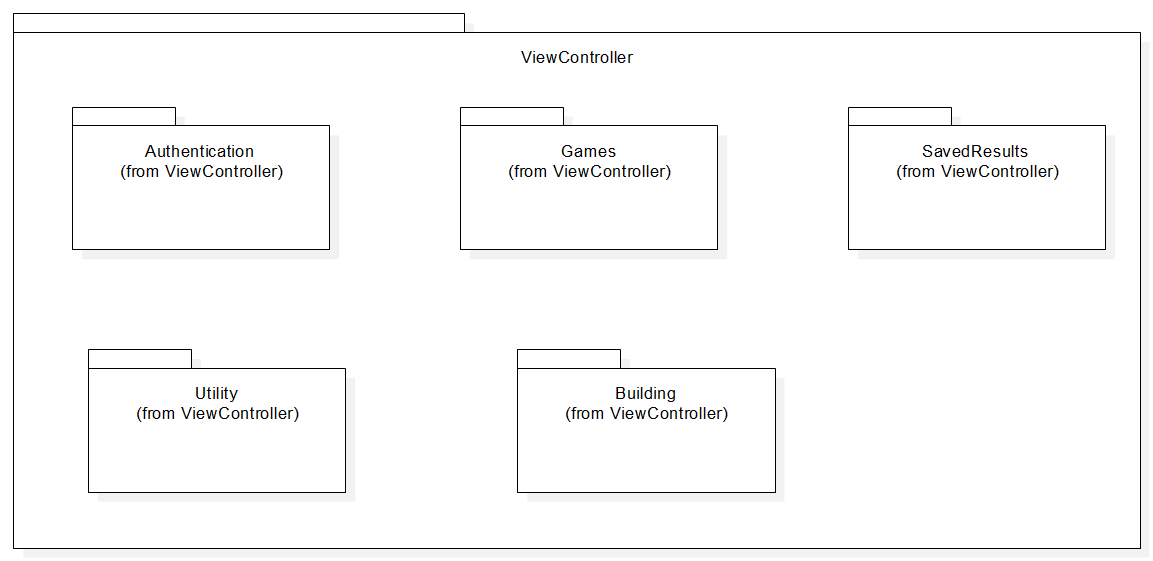
\includegraphics[scale=0.4]{img/package/png/client--viewcontroller.png} 
\caption{Schema package client::viewcontroller} 
 \end{figure} 
\compDescrizione{componente che raggruppa tutte le view ed i controller relativi alle view}
\compPadre{client}
\begin{compPackageContenuti}
\item CLIPS::client::viewcontroller::authentication: componente che si occupa di gestire l'autenticazione dell'utente
\item CLIPS::client::viewcontroller::building: componente che gestisce le informazioni e le interazioni dell'utente con gli edifici abilitati
\item CLIPS::client::viewcontroller::games: componente che gestisce le prove che l'utente deve completare all'interno di un percorso
\item CLIPS::client::viewcontroller::savedresults: componente che raggruppa le le view e i controller dei risultati salvati e delle classifiche
\item CLIPS::client::viewcontroller::utility: componente che raggruppa le view generali dell'app
\end{compPackageContenuti}
\begin{compClassi} \\ 
\begin{classe}{CLIPS::client::viewcontroller::ResultAdapter}
\classeDescrizione{classe che permette la corretta visualizzazione dei risultati di un utente}
\classeUtilizzo{viene usata da SavedResultActivity}
\end{classe}\end{compClassi}
\end{componente}
\begin{componente}{CLIPS::client::viewcontroller::authentication}
\begin{figure}[h!]
	\centering
	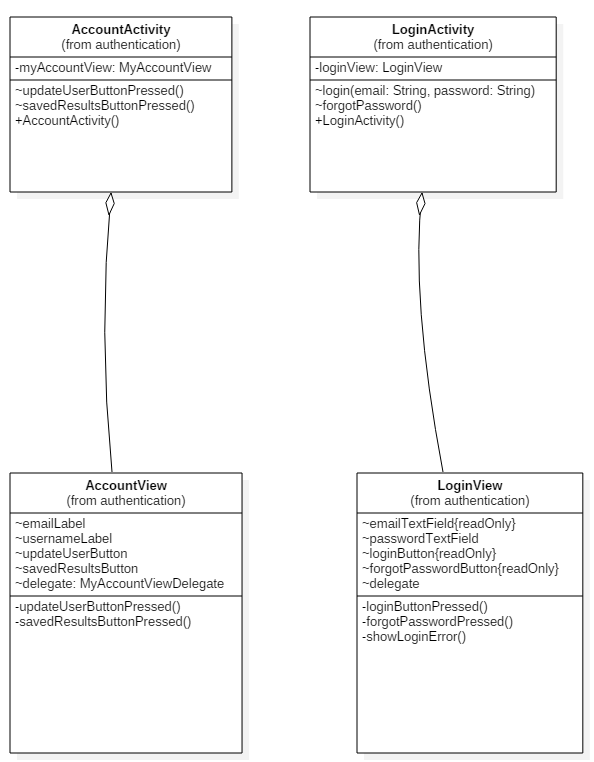
\includegraphics[scale=0.4]{img/package/png/client--viewcontroller--authentication1.png}
	\caption{Prima parte schema package client::viewcontroller::authentication}
\end{figure}
\begin{figure}[h!]
	\centering
	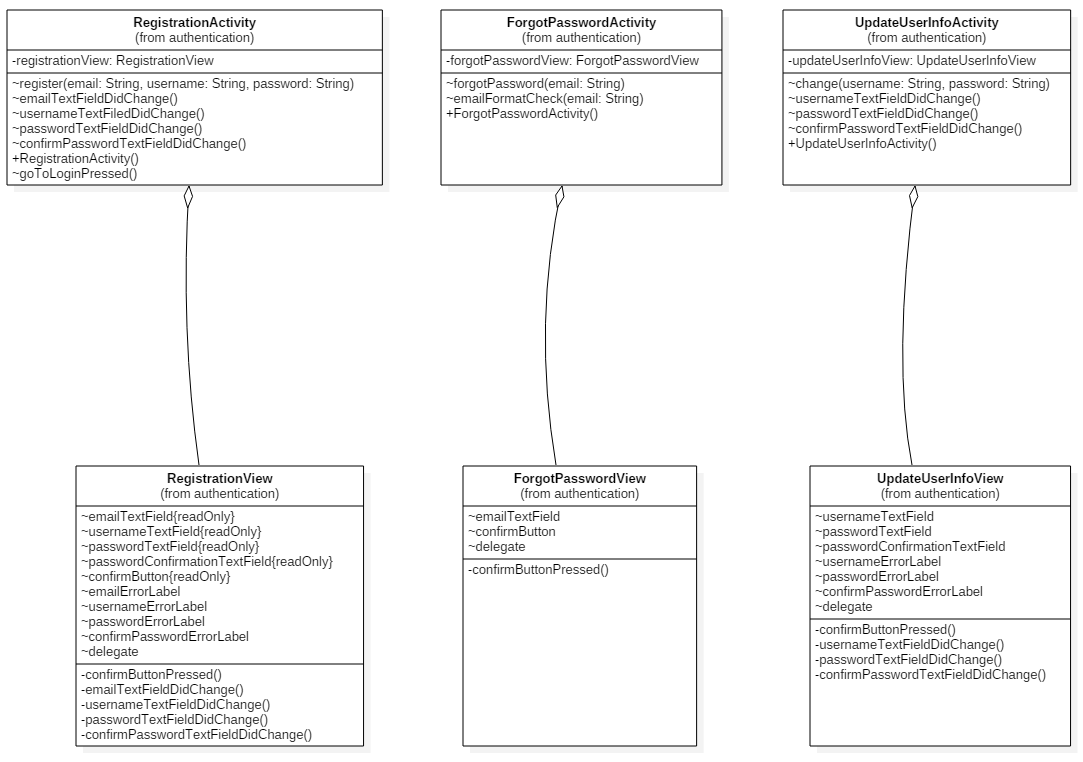
\includegraphics[scale=0.4]{img/package/png/client--viewcontroller--authentication2.png}
	\caption{Seconda parte schema package client::viewcontroller::authentication}
\end{figure} 
\compDescrizione{componente che si occupa di gestire l'autenticazione dell'utente}
\compPadre{viewcontroller}
\begin{compClassi} \\ 
\begin{classe}{CLIPS::client::viewcontroller::authentication::AccountActivity}
\classeDescrizione{classe controller che si occupa di interagire con AccountView}
\classeUtilizzo{si occupa di gestire le interazioni dell'utente con AccountView}
\end{classe}\begin{classe}{CLIPS::client::viewcontroller::authentication::AccountView}
\classeDescrizione{classe che rappresenta la schermata delle informazioni dell'utente}
\classeUtilizzo{permette all'utente di visualizzare le informazioni del proprio profilo}
\begin{classeRelazioni}
\classeRelazione{CLIPS::client::viewcontroller::authentication}{AccountActivity}{classe controller che si occupa di interagire con AccountView}\end{classeRelazioni}
\end{classe}\begin{classe}{CLIPS::client::viewcontroller::authentication::ChangeProfileActivity}
\classeDescrizione{permette all'utente di cambiare le proprie credenziali }
\classeUtilizzo{l'utente grazie a ChangeProfileView potrà cambiare le proprie credenziali}
\end{classe}\begin{classe}{CLIPS::client::viewcontroller::authentication::ConfirmRegistration}
\classeDescrizione{classe che interagisce con RegistrationActivity e permette all'utente di visualizzare i propri dati di registrazione}
\classeUtilizzo{l'utente può visualizzare i dati inseriti in precedenza}
\begin{classeRelazioni}
\classeRelazione{CLIPS::client::viewcontroller::authentication}{RegistrationActivity}{classe controller che si occupa di interagire con RegistrationView}\end{classeRelazioni}
\end{classe}\begin{classe}{CLIPS::client::viewcontroller::authentication::ForgotPasswordActivity}
\classeDescrizione{classe controller che si occupa di interagire con ForgotPasswordView}
\classeUtilizzo{si occupa di gestire le interazioni dell'utente con ForgotPasswordView}
\begin{classeRelazioni}
\classeRelazione{CLIPS::client::viewcontroller::authentication}{ForgotPasswordView}{classe che si occupa della visualizzazione della schermata per la richiesta di una nuova password}\end{classeRelazioni}
\end{classe}\begin{classe}{CLIPS::client::viewcontroller::authentication::ForgotPasswordView}
\classeDescrizione{classe che si occupa della visualizzazione della schermata per la richiesta di una nuova password}
\classeUtilizzo{consente all'utente di inserire la mail per ricevere una nuova password}
\end{classe}\begin{classe}{CLIPS::client::viewcontroller::authentication::LoginActivity}
\classeDescrizione{classe controller che si occupa di interagire con LoginView}
\classeUtilizzo{si occupa di gestire le interazioni dell'utente con LoginView}
\begin{classeRelazioni}
\classeRelazione{CLIPS::client::viewcontroller::authentication}{LoginView}{classe che si occupa della visualizzazione della schermata per il login}\end{classeRelazioni}
\end{classe}\begin{classe}{CLIPS::client::viewcontroller::authentication::LoginView}
\classeDescrizione{classe che si occupa della visualizzazione della schermata per il login}
\classeUtilizzo{consente all'utente di inserire i propri dati per effettuare il login}
\end{classe}\begin{classe}{CLIPS::client::viewcontroller::authentication::RecoverPassword}
\classeDescrizione{classe che rappresenta l'avvenuto recupero della password di un utente}
\classeUtilizzo{view che permette all'utente di sapere che la sua password è stata recuperata correttamente}
\end{classe}\begin{classe}{CLIPS::client::viewcontroller::authentication::RegistrationActivity}
\classeDescrizione{classe controller che si occupa di interagire con RegistrationView}
\classeUtilizzo{si occupa di gestire le interazioni dell'utente con RegistrationView}
\begin{classeRelazioni}
\classeRelazione{CLIPS::client::viewcontroller::authentication}{RegistrationView}{classe che si occupa della visualizzazione della schermata per la registrazione}\end{classeRelazioni}
\end{classe}\begin{classe}{CLIPS::client::viewcontroller::authentication::RegistrationView}
\classeDescrizione{classe che si occupa della visualizzazione della schermata per la registrazione}
\classeUtilizzo{consente all'utente di inserire i propri dati per effettuare la registrazione}

\end{classe}\begin{classe}{CLIPS::client::viewcontroller::authentication::UpdateUserInfoActivity}
\classeDescrizione{classe controller che si occupa di interagire con UpdateUserInfoView}
\classeUtilizzo{si occupa di gestire le interazioni dell'utente con UpdateUserInfoView}
\begin{classeRelazioni}
\classeRelazione{CLIPS::client::viewcontroller::authentication}{UpdateUserInfoView}{classe che si occupa della visualizzazione della schermata per il cambio delle credenziali}\end{classeRelazioni}
\end{classe}\begin{classe}{CLIPS::client::viewcontroller::authentication::UpdateUserInfoView}
\classeDescrizione{classe che si occupa della visualizzazione della schermata per il cambio delle credenziali}
\classeUtilizzo{consente all'utente di inserire i nuovi dati per cambiare le sue credenziali}
\end{classe}\end{compClassi}
\end{componente}
\begin{componente}{CLIPS::client::viewcontroller::building}
\begin{figure}[h!] 
\centering 
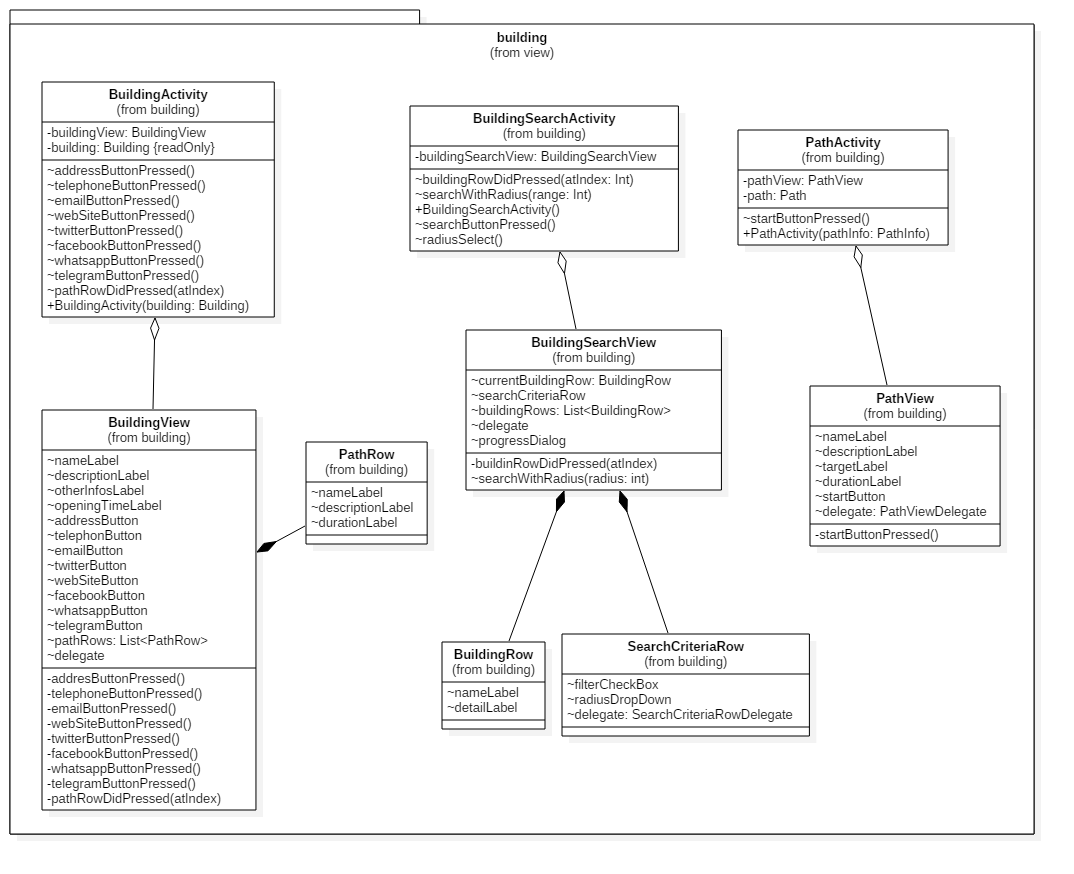
\includegraphics[scale=0.4]{img/package/png/client--viewcontroller--building.png} 
\caption{Schema package client::viewcontroller::building} 
 \end{figure} 
\compDescrizione{componente che gestisce le informazioni e le interazioni dell'utente con gli edifici abilitati}
\compPadre{viewcontroller}
\begin{compClassi} \\ 
\begin{classe}{CLIPS::client::viewcontroller::building::BuildingActivity}
\classeDescrizione{classe controller che si occupa di interagire con BuildingView}
\classeUtilizzo{classe controller che si occupa di interagire con BuildingView}
\begin{classeRelazioni}
\classeRelazione{CLIPS::client::viewcontroller::building}{BuildingView}{classe per la visualizzazione di un edificio}\end{classeRelazioni}
\end{classe}\begin{classe}{CLIPS::client::viewcontroller::building::BuildingRow}
\classeDescrizione{classe per la rappresentazione di un edificio nella ricerca}
\classeUtilizzo{permette di visualizzare le informazioni di un edificio nella lista dei risultati di ricerca}
\end{classe}\begin{classe}{CLIPS::client::viewcontroller::building::BuildingSearchActivity}
\classeDescrizione{classe controller che si occupa di interagire con BuildingSearchView}
\classeUtilizzo{si occupa di gestire le interazioni dell'utente con BuildingSearchView}
\begin{classeRelazioni}
\classeRelazione{CLIPS::client::viewcontroller::building}{BuildingSearchView}{classe per la ricerca degli edifici}\end{classeRelazioni}
\end{classe}\begin{classe}{CLIPS::client::viewcontroller::building::BuildingSearchView}
\classeDescrizione{classe per la ricerca degli edifici}
\classeUtilizzo{permette all'utente di cercare gli edifici vicini per visualizzare le informazioni e/o i percorsi disponibili}

\begin{classeRelazioni}
\classeRelazione{CLIPS::client::viewcontroller::building}{BuildingRow}{classe per la rappresentazione di un edificio nella ricerca}\classeRelazione{CLIPS::client::viewcontroller::building}{SearchCriteriaRow}{classe utilizzata per determinare i criteri di ricerca degli edifici}\end{classeRelazioni}
\end{classe}\begin{classe}{CLIPS::client::viewcontroller::building::BuildingView}
\classeDescrizione{classe per la visualizzazione di un edificio}
\classeUtilizzo{permette all'utente di visualizzare le informazioni relative all'edificio selezionato}
\begin{classeRelazioni}
\classeRelazione{CLIPS::client::viewcontroller::building}{PathRow}{classe per la rappresentazione di un percorso nella ricerca}\end{classeRelazioni}
\end{classe}\begin{classe}{CLIPS::client::viewcontroller::building::PathActivity}
\classeDescrizione{classe controller che si occupa di interagire con PathView}
\classeUtilizzo{si occupa di gestire le interazioni dell'utente con PathView}
\begin{classeRelazioni}
\classeRelazione{CLIPS::client::viewcontroller::building}{PathView}{classe che si occupa della visualizzazione della schermata riguardante un percorso}\end{classeRelazioni}
\end{classe}\begin{classe}{CLIPS::client::viewcontroller::building::PathRow}
\classeDescrizione{classe per la rappresentazione di un percorso nella ricerca}
\classeUtilizzo{permette un percorso disponibile nella lista dei risultati di ricerca}
\end{classe}\begin{classe}{CLIPS::client::viewcontroller::building::PathView}
\classeDescrizione{classe che si occupa della visualizzazione della schermata riguardante un percorso}
\classeUtilizzo{consente all'utente di visualizzare le informazioni riguardanti un percorso e se l'utente si trova nell'edificio del percorso consente di iniziarlo}
\end{classe}\begin{classe}{CLIPS::client::viewcontroller::building::SearchCriteriaRow}
\classeDescrizione{classe utilizzata per determinare i criteri di ricerca degli edifici}
\classeUtilizzo{permette all'utente di visualizzare i criteri di ricerca disponibili}
\end{classe}\end{compClassi}
\end{componente}
\begin{componente}{CLIPS::client::viewcontroller::games}
\begin{figure}[h!]
	\centering
	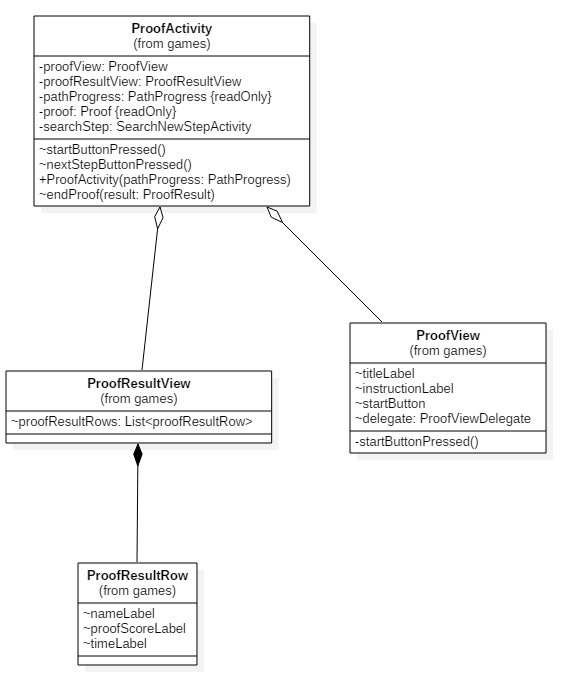
\includegraphics[scale=0.5]{img/package/png/client--viewcontroller--games1.png}
	\caption{Prima parte schema package client::viewcontroller::games}
\end{figure}
\begin{figure}[h!]
	\centering
	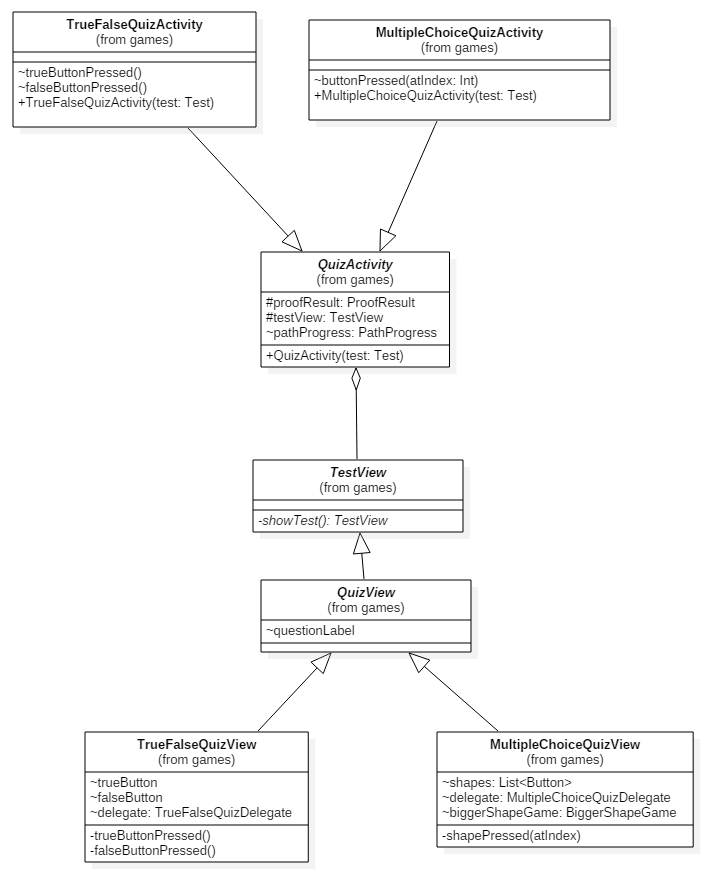
\includegraphics[scale=0.5]{img/package/png/client--viewcontroller--games2.png}
	\caption{Seconda parte schema package client::viewcontroller::games}
\end{figure}
\begin{figure}[h!]
	\centering
	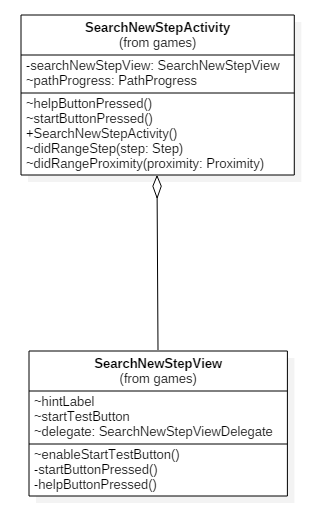
\includegraphics[scale=0.5]{img/package/png/client--viewcontroller--games3.png}
	\caption{Terza parte schema package client::viewcontroller::games}
\end{figure} 
\compDescrizione{componente che gestisce le prove che l'utente deve completare all'interno di un percorso}
\compPadre{viewcontroller}
\begin{compClassi} \\ 
\begin{classe}{CLIPS::client::viewcontroller::games::MultipleChoiceQuizActivity}
\classeDescrizione{classe controller che si occupa di interagire con MultipleChoiceView}
\classeUtilizzo{si occupa di gestire le interazioni dell'utente con MultipleChoiceView}
\begin{classeRelazioni}
\classeRelazione{CLIPS::client::viewcontroller::games}{QuizActivity}{interfaccia per segnalare gli eventi della classe QuizView}\end{classeRelazioni}
\end{classe}\begin{classe}{CLIPS::client::viewcontroller::games::MultipleChoiceQuizView}
\classeDescrizione{classe per il quiz a risposta multipla}
\classeUtilizzo{si occupa di fornire un'interfaccia per il quiz a risposta multipla}
\begin{classeRelazioni}
\classeRelazione{CLIPS::client::viewcontroller::games}{QuizView}{classe base per i quiz}\end{classeRelazioni}
\end{classe}\begin{classe}{CLIPS::client::viewcontroller::games::ProofActivity}
\classeDescrizione{classe controller che si occupa di interagire con ProofView}
\classeUtilizzo{si occupa di gestire le interazioni dell'utente con ProofView}
\begin{classeRelazioni}
\classeRelazione{CLIPS::client::viewcontroller::games}{ProofResultView}{classe che rappresenta la schermata dei risultati}\end{classeRelazioni}
\end{classe}\begin{classe}{CLIPS::client::viewcontroller::games::ProofResultActivity}
\classeDescrizione{classe che permette di visualizzare il risultato di una prova}
\classeUtilizzo{l'utente può vedere il risultato della prova che  ha appena svolto}
\end{classe}\begin{classe}{CLIPS::client::viewcontroller::games::ProofResultRow}
\classeDescrizione{classe che rappresenta una risultato rappresentato all'interno di una riga che può essere cliccata}
\classeUtilizzo{permette all'utente di visualizzare le informazioni generali di un risultato di una prova e di cliccarci per visualizzarne le informazioni dettagliate}
\end{classe}\begin{classe}{CLIPS::client::viewcontroller::games::ProofResultView}
\classeDescrizione{classe che rappresenta la schermata dei risultati}
\classeUtilizzo{permette all'utente di visualizzare le informazioni generali dei risultati delle prove e cliccare sulle prove delle quali vuole visualizzare le informazioni dettagliate}
\begin{classeRelazioni}
\classeRelazione{CLIPS::client::viewcontroller::games}{ProofResultRow}{classe che rappresenta una risultato rappresentato all'interno di una riga che può essere cliccata}\end{classeRelazioni}
\end{classe}\begin{classe}{CLIPS::client::viewcontroller::games::ProofView}
\classeDescrizione{classe che rappresenta la schermata della prova}
\classeUtilizzo{permette all'utente di visualizzare la prova da giocare}
\end{classe}\begin{classe}{CLIPS::client::viewcontroller::games::QuizActivity}
\classeDescrizione{interfaccia per segnalare gli eventi della classe QuizView}
\classeUtilizzo{si occupa di fornire i metodi necessari alla classe QuizView per notificare gli eventi}
\end{classe}\begin{classe}{CLIPS::client::viewcontroller::games::QuizResultView}
\classeDescrizione{classe per la visualizzazione del risultato di un quiz}
\classeUtilizzo{fornisce all'utente un'interfaccia affinché visualizzi il risultato del quiz}
\end{classe}\begin{classe}{CLIPS::client::viewcontroller::games::QuizView}
\classeDescrizione{classe base per i quiz}
\classeUtilizzo{fornisce una base per i vari tipi di test da istanziare}
\begin{classeRelazioni}
\classeRelazione{CLIPS::client::viewcontroller::games}{TestView}{classe che fornisce una base dalla quale è possibile creare vari tipi di giochi }\end{classeRelazioni}
\end{classe}\begin{classe}{CLIPS::client::viewcontroller::games::SearchNewStepActivity}
\classeDescrizione{classe controller che si occupa di interagire con SearchNewStepView}
\classeUtilizzo{si occupa di gestire le interazioni dell'utente con SearchNewStepView}
\begin{classeRelazioni}
\classeRelazione{CLIPS::client::viewcontroller::games}{SearchNewStepView}{classe che rappresenta la schermata per la ricerca della prossima prova del percorso}\end{classeRelazioni}
\end{classe}\begin{classe}{CLIPS::client::viewcontroller::games::SearchNewStepView}
\classeDescrizione{classe che rappresenta la schermata per la ricerca della prossima prova del percorso}
\classeUtilizzo{permette all'utente di cercare in modo semplificato la ricerca della prossima prova del percorso}
\end{classe}\begin{classe}{CLIPS::client::viewcontroller::games::TestResultView}
\classeDescrizione{classe che fornisce una base per la visualizzazione del risultato della prova}
\classeUtilizzo{permette all'utente di visualizzare il risultato della prova}
\end{classe}\begin{classe}{CLIPS::client::viewcontroller::games::TestView}
\classeDescrizione{classe che fornisce una base dalla quale è possibile creare vari tipi di giochi }
\classeUtilizzo{viene utilizzata per visualizzare un'interfaccia di gioco all'utente}
\end{classe}\begin{classe}{CLIPS::client::viewcontroller::games::TrueFalseQuizActivity}
\classeDescrizione{classe controller che si occupa di interagire con TrueFalseQuizView}
\classeUtilizzo{si occupa di gestire le interazioni dell'utente con TrueFalseQuizView}
\begin{classeRelazioni}
\classeRelazione{CLIPS::client::viewcontroller::games}{QuizActivity}{interfaccia per segnalare gli eventi della classe QuizView}\end{classeRelazioni}
\end{classe}\begin{classe}{CLIPS::client::viewcontroller::games::TrueFalseQuizView}
\classeDescrizione{classe per il quiz vero/falso}
\classeUtilizzo{si occupa di fornire un'interfaccia per la prova di tipo vero/falso}
\begin{classeRelazioni}
\classeRelazione{CLIPS::client::viewcontroller::games}{QuizView}{classe base per i quiz}\end{classeRelazioni}
\end{classe}\end{compClassi}
\end{componente}
\begin{componente}{CLIPS::client::viewcontroller::savedresults}
\begin{figure}[h!] 
\centering 
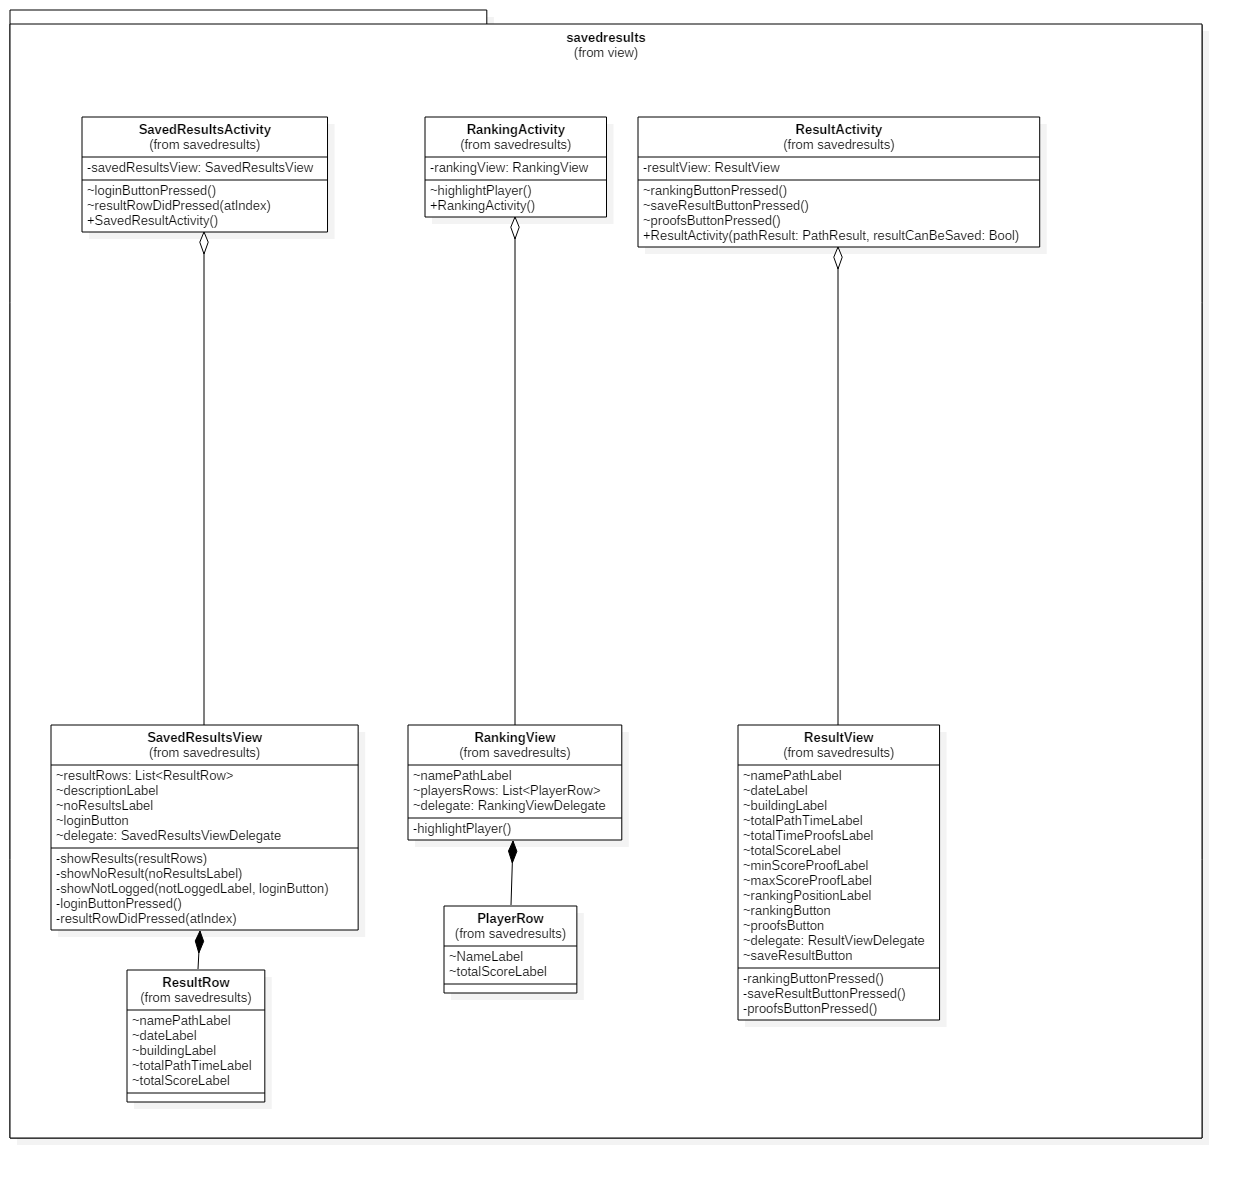
\includegraphics[scale=0.4]{img/package/png/client--viewcontroller--savedresults.png} 
\caption{Schema package client::viewcontroller::savedresults} 
 \end{figure} 
\compDescrizione{componente che raggruppa le le view e i controller dei risultati salvati e delle classifiche}
\compPadre{viewcontroller}
\begin{compClassi} \\ 
\begin{classe}{CLIPS::client::viewcontroller::savedresults::PlayerRow}
\classeDescrizione{classe che rappresenta una riga all'interno di una classifica}
\classeUtilizzo{permette all'utente di visualizzare il nome del giocatore e il suo punteggio nel percorso d'interesse}
\end{classe}\begin{classe}{CLIPS::client::viewcontroller::savedresults::RankingActivity}
\classeDescrizione{classe controller che si occupa di interagire con RankingView}
\classeUtilizzo{si occupa di gestire le interazioni dell'utente con RankingView}
\end{classe}\begin{classe}{CLIPS::client::viewcontroller::savedresults::RankingView}
\classeDescrizione{classe per rappresentare la classifica di un percorso}
\classeUtilizzo{permette all'utente di visualizzare la classifica del percorso}
\begin{classeRelazioni}
\classeRelazione{CLIPS::client::viewcontroller::savedresults}{RankingActivity}{classe controller che si occupa di interagire con RankingView}\end{classeRelazioni}
\end{classe}\begin{classe}{CLIPS::client::viewcontroller::savedresults::ResultActivity}
\classeDescrizione{classe controller che si occupa di interagire con ResultView}
\classeUtilizzo{si occupa di gestire le interazioni dell'utente con ResultView}
\begin{classeRelazioni}
\classeRelazione{CLIPS::client::viewcontroller::savedresults}{ResultView}{classe che rappresenta la schermata nel quali si possono visualizzare i risultati di un percorso}\classeRelazione{CLIPS::client::viewcontroller::savedresults}{ResultView}{classe che rappresenta la schermata nel quali si possono visualizzare i risultati di un percorso}\end{classeRelazioni}
\end{classe}\begin{classe}{CLIPS::client::viewcontroller::savedresults::ResultRow}
\classeDescrizione{classe che rappresenta una riga di un risultato}
\classeUtilizzo{permette all'utente di visualizzare le informazioni generali di un risultato e di cliccarci per visualizzare quelle dettagliate}
\end{classe}\begin{classe}{CLIPS::client::viewcontroller::savedresults::ResultView}
\classeDescrizione{classe che rappresenta la schermata nel quali si possono visualizzare i risultati di un percorso}
\classeUtilizzo{permette all'utente di visualizzare le informazioni dettagliate del risultato di un percorso}
\end{classe}\begin{classe}{CLIPS::client::viewcontroller::savedresults::SavedResultsActivity}
\classeDescrizione{classe controller che si occupa di interagire con SavedResultView}
\classeUtilizzo{si occupa di gestire le interazioni dell'utente con SavedResultView}
\begin{classeRelazioni}
\classeRelazione{CLIPS::client::viewcontroller::savedresults}{SavedResultView}{classe che rappresenta la schermata dei risultati salvati di un utente}\end{classeRelazioni}
\end{classe}\begin{classe}{CLIPS::client::viewcontroller::savedresults::SavedResultView}
\classeDescrizione{classe che rappresenta la schermata dei risultati salvati di un utente}
\classeUtilizzo{permette all'utente di visualizzare i propri risultati salvati}
\begin{classeRelazioni}
\classeRelazione{CLIPS::client::viewcontroller::savedresults}{ResultRow}{classe che rappresenta una riga di un risultato}\end{classeRelazioni}
\end{classe}\end{compClassi}
\end{componente}
\begin{componente}{CLIPS::client::viewcontroller::utility}
\begin{figure}[h!] 
\centering 
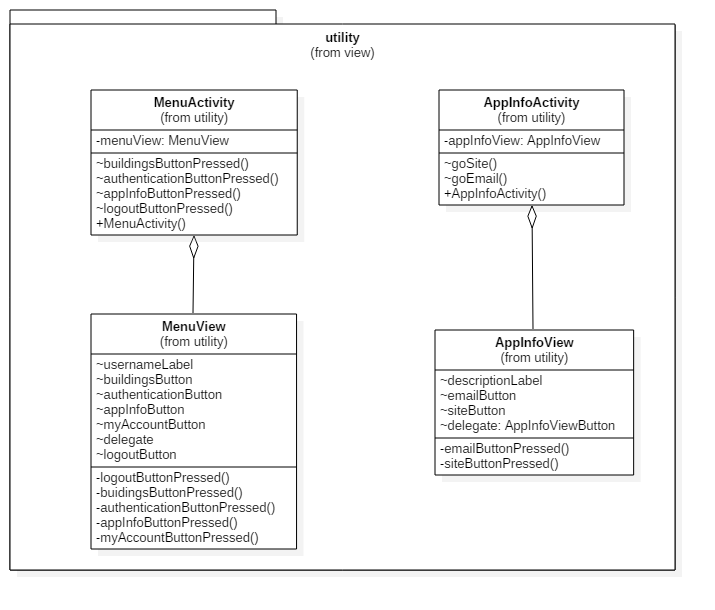
\includegraphics[scale=0.4]{img/package/png/client--viewcontroller--utility.png} 
\caption{Schema package client::viewcontroller::utility} 
 \end{figure} 
\compDescrizione{componente che raggruppa le view generali dell'app}
\compPadre{viewcontroller}
\begin{compClassi} \\ 
\begin{classe}{CLIPS::client::viewcontroller::utility::AppInfoActivity}
\classeDescrizione{classe controller che si occupa di interagire con AppInfoView}
\classeUtilizzo{si occupa di gestire le interazioni dell'utente con AppInfoView}
\begin{classeRelazioni}
\classeRelazione{CLIPS::client::viewcontroller::utility}{AppInfoView}{classe che si occupa delle informazioni generali dell'app}\end{classeRelazioni}
\end{classe}\begin{classe}{CLIPS::client::viewcontroller::utility::AppInfoView}
\classeDescrizione{classe che si occupa delle informazioni generali dell'app}
\classeUtilizzo{permette all'utente di visualizzare le informazioni generali dell'app}
\end{classe}\begin{classe}{CLIPS::client::viewcontroller::utility::MenuActivity}
\classeDescrizione{classe controller che si occupa di interagire con MenuView}
\classeUtilizzo{si occupa di gestire le interazioni dell'utente con MenuView}

\begin{classeRelazioni}
\classeRelazione{CLIPS::client::viewcontroller::utility}{MenuView}{classe che si occupa di far visualizzare il menu}\end{classeRelazioni}
\end{classe}\begin{classe}{CLIPS::client::viewcontroller::utility::MenuView}
\classeDescrizione{classe che si occupa di far visualizzare il menu}
\classeUtilizzo{consente all'utente di navigare nell'app tramite il menu}
\end{classe}\end{compClassi}
\end{componente}
\begin{componente}{CLIPS::server}
\begin{figure}[h!] 
\centering 
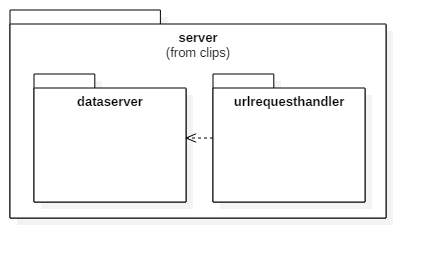
\includegraphics[scale=0.4]{img/package/png/server.png} 
\caption{Schema package server} 
 \end{figure} 
\compDescrizione{componente globale per il back end del prodotto}
\compPadre{CLIPS}
\begin{compPackageContenuti}
\item CLIPS::server::dataserver: package per la gestione dei dati sul server
\item CLIPS::server::urlrequesthandler: componente che gestisce le richieste inviate al server e le risposte da inviare al client
\end{compPackageContenuti}
\end{componente}
\begin{componente}{CLIPS::server::dataserver}
\begin{figure}[h!] 
\centering 
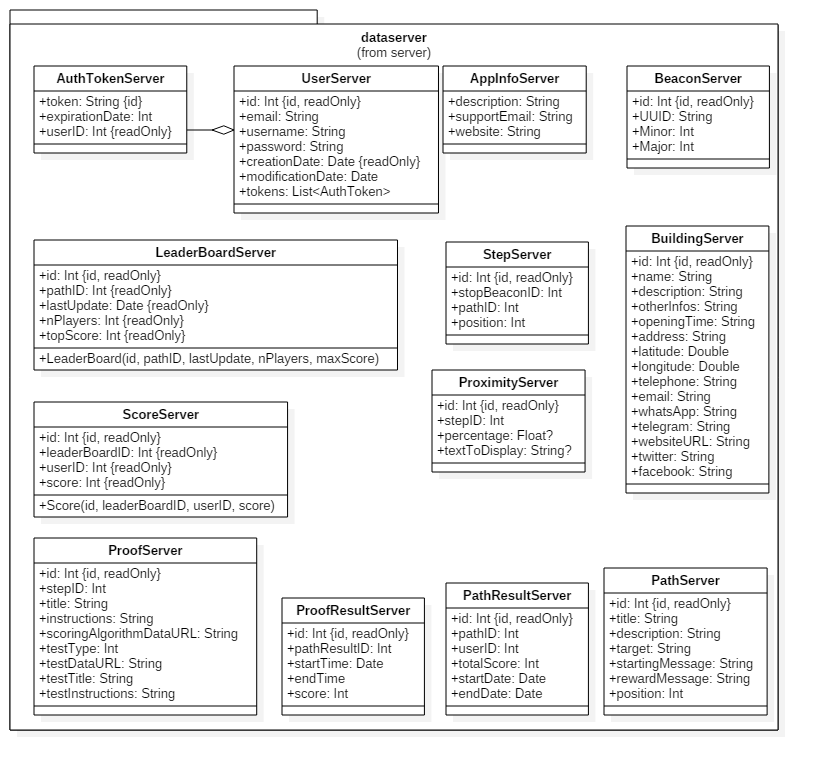
\includegraphics[scale=0.4]{img/package/png/server--data.png} 
\caption{Schema package server::dataserver} 
 \end{figure} 
\compDescrizione{package per la gestione dei dati sul server}
\compPadre{server}
\begin{compClassi} \\ 
\begin{classe}{CLIPS::server::dataserver::AppInfoServer}
\classeDescrizione{classe che rappresenta le informazioni dell'app sul server}
\classeUtilizzo{permette di salvare sul server le informazioni dell'app}
\end{classe}\begin{classe}{CLIPS::server::dataserver::AuthTokenServer}
\classeDescrizione{Classe che rappresenta un token che si riferisce ad un utente loggato}
\classeUtilizzo{permette utilizzare un token per riferirsi ad utente loggato}
\end{classe}\begin{classe}{CLIPS::server::dataserver::BeaconServer}
\classeDescrizione{classe che rappresenta un beacon nel server}
\classeUtilizzo{permette di salvare sul server un beacon}
\end{classe}\begin{classe}{CLIPS::server::dataserver::BuildingServer}
\classeDescrizione{classe che rappresenta un edificio sul server}
\classeUtilizzo{permette di salvare e modificare i dati di un edificio sul server}
\end{classe}\begin{classe}{CLIPS::server::dataserver::LeaderBoardServer}
\classeDescrizione{classe che rappresenta la classifica sul server}
\classeUtilizzo{permette di salvare i dati della classifica sul server}
\end{classe}\begin{classe}{CLIPS::server::dataserver::PathResultServer}
\classeDescrizione{classe che rappresenta il risultato di un percorso sul server}
\classeUtilizzo{consente di salvare i risultati di un percorso sul server}
\end{classe}\begin{classe}{CLIPS::server::dataserver::PathServer}
\classeDescrizione{classe che rappresenta un percorso sul server}
\classeUtilizzo{permette di creare, modificare ed eliminare un percorso sul server}
\end{classe}\begin{classe}{CLIPS::server::dataserver::ProofResultServer}
\classeDescrizione{classe che rappresenta i risultati di una prova sul server}
\classeUtilizzo{consente di salvare il risultato di una prova sul server}
\end{classe}\begin{classe}{CLIPS::server::dataserver::ProofServer}
\classeDescrizione{classe che rappresenta una prova sul server}
\classeUtilizzo{permette di creare, modificare ed eliminare una prova sul server}
\end{classe}\begin{classe}{CLIPS::server::dataserver::ProximityServer}
\classeDescrizione{classe che rappresenta sul server un beacon indicato alla segnalazione della distanza dalla prossima prova}
\classeUtilizzo{permette di salvare i beacon di segnalazione sul server}
\end{classe}\begin{classe}{CLIPS::server::dataserver::ScoreManager}
\classeDescrizione{classe che rappresenta un risultato sul server}
\classeUtilizzo{permette si salvare un risultato nel server}
\end{classe}\begin{classe}{CLIPS::server::dataserver::StepServer}
\classeDescrizione{classe che rappresenta uno step di un percorso nel server}
\classeUtilizzo{permette di salvare sul server uno step di un percorso}
\end{classe}\begin{classe}{CLIPS::server::dataserver::UserServer}
\classeDescrizione{classe che rappresenta un utente nel server}
\classeUtilizzo{permette di salvare sul server un utente}
\begin{classeRelazioni}
\classeRelazione{CLIPS::server::dataserver}{AuthTokenServer}{Classe che rappresenta un token che si riferisce ad un utente loggato}\end{classeRelazioni}
\end{classe}\end{compClassi}
\end{componente}
\begin{componente}{CLIPS::server::urlrequesthandler}
\begin{figure}[h!] 
\centering 
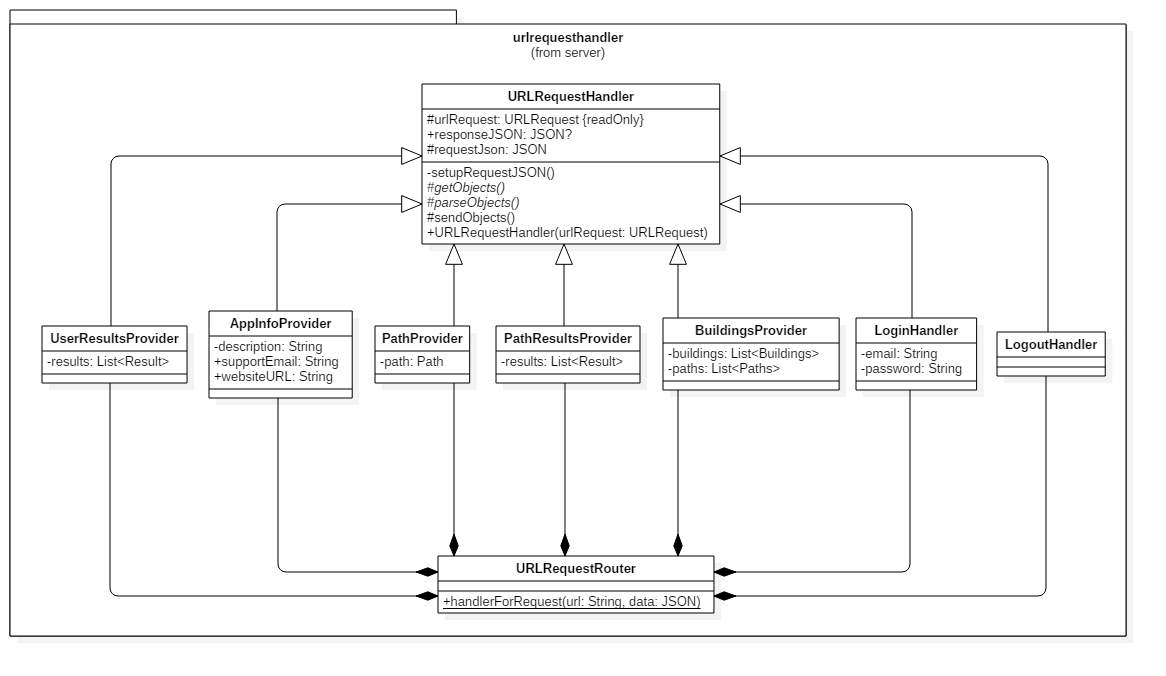
\includegraphics[scale=0.4]{img/package/png/server--urlrequesthandler.png} 
\caption{Schema package server::urlrequesthandler} 
 \end{figure} 
\compDescrizione{componente che gestisce le richieste inviate al server e le risposte da inviare al client}
\compPadre{server}
\begin{compClassi} \\ 
\begin{classe}{CLIPS::server::urlrequesthandler::AppInfoProvider}
\classeDescrizione{classe che gestisce la richiesta di informazioni sull'app (come la descrizione dell'app, l'indirizzo del sito di supporto, l'email del supporto tecnico ed altro)}
\classeUtilizzo{si occupa di restituire le informazioni dell'app richieste}
\end{classe}\begin{classe}{CLIPS::server::urlrequesthandler::BuildingsProvider}
\classeDescrizione{classe che gestisce la richiesta degli edifici dal client al server}
\classeUtilizzo{si occupa di restituire le informazioni sugli edifici richieste}
\begin{classeRelazioni}
\classeRelazione{CLIPS::server::urlrequesthandler}{DBHandler}{classe che si occupa di gestire il DB e di ritornare un oggetto configurato della libreria knex}\end{classeRelazioni}
\end{classe}\begin{classe}{CLIPS::server::urlrequesthandler::DBHandler}
\classeDescrizione{classe che si occupa di gestire il DB e di ritornare un oggetto configurato della libreria knex}
\classeUtilizzo{creando un oggetto di questa classe è possibile creare query per interagire con il database}
\end{classe}\begin{classe}{CLIPS::server::urlrequesthandler::EmailChecker}
\classeDescrizione{fornisce i metodi per la validazione di un indirizzo email}
\classeUtilizzo{attraverso il metodo isValid(string) è possibile controllare se l'indirizzo email passato in input è valido}
\end{classe}\begin{classe}{CLIPS::server::urlrequesthandler::EmailSender}
\classeDescrizione{classe usata dal server per inviare un email}
\classeUtilizzo{si occupa di inviare un'email da beaconstrips.swe@gmail.com}
\end{classe}\begin{classe}{CLIPS::server::urlrequesthandler::GetUserData}
\classeDescrizione{classe del server che gestisce la richiesta dei dati utente}
\classeUtilizzo{si occupa di tornare al client i dati sull'utente che ha effettuato la chiamata}
\end{classe}\begin{classe}{CLIPS::server::urlrequesthandler::LoginHandler}
\classeDescrizione{classe che gestisce le richieste di login da parte del client}
\classeUtilizzo{si occupa di gestire il login lato server}
\begin{classeRelazioni}
\classeRelazione{CLIPS::server::urlrequesthandler}{DBHandler}{classe che si occupa di gestire il DB e di ritornare un oggetto configurato della libreria knex}\end{classeRelazioni}
\end{classe}\begin{classe}{CLIPS::server::urlrequesthandler::LogoutHandler}
\classeDescrizione{classe che gestisce la richiesta di logout da parte del client (eliminando il token associato al client)}
\classeUtilizzo{si occupa di effettuare il logout lato server}
\end{classe}\begin{classe}{CLIPS::server::urlrequesthandler::PasswordChecker}
\classeDescrizione{verifica che la password soddisfi i requisiti minimi di sicurezza}
\classeUtilizzo{utilizzare il metodo isValid(string) per verificare la sicurezza sufficiente della password inserita}
\end{classe}\begin{classe}{CLIPS::server::urlrequesthandler::PasswordResetEmailSender}
\classeDescrizione{classe che invia una email contenente i dettagli per il reset di una password dimenticata}
\classeUtilizzo{si occupa di notificare l'utente della nuova password impostata dopo averne chiesto il ripristino}
\end{classe}\begin{classe}{CLIPS::server::urlrequesthandler::PasswordResetHandler}
\classeDescrizione{classe del server per gestire la richiesta di reset di una password dimenticata}
\classeUtilizzo{si occupa di verificare se l'indirizzo email fornito corrisponde con quello di qualche account ed eventualmente di resecare la password ed inviare una mail di avvenuto ripristino}
\end{classe}\begin{classe}{CLIPS::server::urlrequesthandler::PathProvider}
\classeDescrizione{classe che gestisce la richiesta del percorso dal client}
\classeUtilizzo{si occupa di restituire le informazioni sul percorso richieste}
\begin{classeRelazioni}
\classeRelazione{CLIPS::server::urlrequesthandler}{DBHandler}{classe che si occupa di gestire il DB e di ritornare un oggetto configurato della libreria knex}\end{classeRelazioni}
\end{classe}\begin{classe}{CLIPS::server::urlrequesthandler::PathResultsProvider}
\classeDescrizione{classe che gestisce la richiesta del risultato del percorso dal client}
\classeUtilizzo{si occupa di restituire le informazioni del risultato sul percorso richieste}
\begin{classeRelazioni}
\classeRelazione{CLIPS::server::urlrequesthandler}{DBHandler}{classe che si occupa di gestire il DB e di ritornare un oggetto configurato della libreria knex}\end{classeRelazioni}
\end{classe}\begin{classe}{CLIPS::server::urlrequesthandler::PostUserData}
\classeDescrizione{classe del server che si occupa della modifica dei dati utente}
\classeUtilizzo{si occupa di modificare nel database i dati dell'utente quando un client chiede che vengano modificati}
\end{classe}\begin{classe}{CLIPS::server::urlrequesthandler::RankingProvider}
\classeDescrizione{provider della classifica per il percorso specificato}
\classeUtilizzo{si occupa di restituire al richiedente la classifica del percorso specificato}
\end{classe}\begin{classe}{CLIPS::server::urlrequesthandler::RegistrationFieldsValidator}
\classeDescrizione{classe del server che si occupa di validare i dati di registrazione}
\classeUtilizzo{la classe presenta un metodo execute che verifica la richiesta effettuata dal client e quali sono i dati forniti e risponde con le indicazioni di quali sono campi validi}
\begin{classeRelazioni}
\classeRelazione{CLIPS::server::urlrequesthandler}{EmailChecker}{fornisce i metodi per la validazione di un indirizzo email}\classeRelazione{CLIPS::server::urlrequesthandler}{PasswordChecker}{verifica che la password soddisfi i requisiti minimi di sicurezza}\classeRelazione{CLIPS::server::urlrequesthandler}{UsernameChecker}{si occupa di verificare la validità dell'username (in particolare se è già in uso da un utente)}\end{classeRelazioni}
\end{classe}\begin{classe}{CLIPS::server::urlrequesthandler::RegistrationHandler}
\classeDescrizione{classe che si occupa di registrare i nuovi utenti}
\classeUtilizzo{è necessario impostare gli attributi response e request e successivamente chiamare il metodo execute()}
\end{classe}\begin{classe}{CLIPS::server::urlrequesthandler::TokenGenerator}
\classeDescrizione{classe per la creazione di stringhe casuali univoche}
\classeUtilizzo{si occupa di creare un token casuale}
\end{classe}\begin{classe}{CLIPS::server::urlrequesthandler::URLRequestHandler}
\classeDescrizione{classe astratta che rappresenta un gestore di richieste di dati fatte al server}
\classeUtilizzo{si occupa di gestire le richieste ricevute dal client}
\end{classe}\begin{classe}{CLIPS::server::urlrequesthandler::URLRequestRouter}
\classeDescrizione{classe che si occupa di creare il corretto URLRequestHandler per gestire la richiesta HTTP rivolta al server}
\classeUtilizzo{crea la classe URLRequestHandler appropriata}
\begin{classeRelazioni}
\classeRelazione{CLIPS::server::urlrequesthandler}{AppInfoProvider}{classe che gestisce la richiesta di informazioni sull'app (come la descrizione dell'app, l'indirizzo del sito di supporto, l'email del supporto tecnico ed altro)}\classeRelazione{CLIPS::server::urlrequesthandler}{BuildingsProvider}{classe che gestisce la richiesta degli edifici dal client al server}\classeRelazione{CLIPS::server::urlrequesthandler}{LoginHandler}{classe che gestisce le richieste di login da parte del client}\classeRelazione{CLIPS::server::urlrequesthandler}{LogoutHandler}{classe che gestisce la richiesta di logout da parte del client (eliminando il token associato al client)}\classeRelazione{CLIPS::server::urlrequesthandler}{PathProvider}{classe che gestisce la richiesta del percorso dal client}\classeRelazione{CLIPS::server::urlrequesthandler}{PathResultsProvider}{classe che gestisce la richiesta del risultato del percorso dal client}\classeRelazione{CLIPS::server::urlrequesthandler}{RegistrationFieldsValidator}{classe del server che si occupa di validare i dati di registrazione}\classeRelazione{CLIPS::server::urlrequesthandler}{UserResultProvider}{classe che gestisce la richiesta di un utente}\end{classeRelazioni}
\end{classe}\begin{classe}{CLIPS::server::urlrequesthandler::UserDataRequest}
\classeDescrizione{classe che si occupa di gestire una richiesta che opera sui dati dell'utente}
\classeUtilizzo{la classe mette a disposizioni delle sottoclassi una varietà di metodi per gestire agevolmente i dati degli utenti}
\end{classe}\begin{classe}{CLIPS::server::urlrequesthandler::UsernameChecker}
\classeDescrizione{si occupa di verificare la validità dell'username (in particolare se è già in uso da un utente)}
\classeUtilizzo{è utile per verificare che un username non sia ancora stato utilizzato}
\end{classe}\begin{classe}{CLIPS::server::urlrequesthandler::UserResultProvider}
\classeDescrizione{classe che gestisce la richiesta di un utente}
\classeUtilizzo{si occupa di restituire gli utenti richiesti dal client}
\end{classe}\end{compClassi}
\end{componente}
